\documentclass[11pt, a4paper]{article}

% ── Packages ──────────────────────────────────────────────
\usepackage[utf8]{inputenc}
\usepackage[T1]{fontenc}
\usepackage{lmodern}
\usepackage[margin=2.5cm]{geometry}
\usepackage{graphicx}
\usepackage{booktabs}
\usepackage{amsmath, amssymb}
\usepackage{hyperref}
\usepackage{cleveref}
\usepackage{caption}
\usepackage{subcaption}
\usepackage{float}
\usepackage{placeins}
\usepackage{enumitem}
\usepackage{xcolor}
\usepackage{microtype}
\usepackage{authblk}
\usepackage{abstract}
\usepackage{titlesec}
\usepackage{parskip}

\graphicspath{{../analytics/}}

% Force figures to stay in their declared section
\let\oldsection\section
\renewcommand{\section}[1]{\FloatBarrier\oldsection{#1}}
\let\oldsubsection\subsection
\renewcommand{\subsection}[1]{\FloatBarrier\oldsubsection{#1}}

\hypersetup{
    colorlinks=true,
    linkcolor=blue!60!black,
    citecolor=blue!60!black,
    urlcolor=blue!60!black,
}

% Tighten spacing
\titlespacing*{\section}{0pt}{1.5ex plus 0.5ex}{0.8ex plus 0.2ex}
\titlespacing*{\subsection}{0pt}{1.2ex plus 0.3ex}{0.6ex plus 0.2ex}
\titlespacing*{\subsubsection}{0pt}{1.0ex plus 0.2ex}{0.4ex plus 0.1ex}
\setlength{\abovecaptionskip}{6pt}
\setlength{\belowcaptionskip}{4pt}
\setlength{\floatsep}{10pt plus 2pt minus 2pt}
\setlength{\textfloatsep}{12pt plus 2pt minus 2pt}

% ── Title ─────────────────────────────────────────────────
\title{\textbf{Seeing the Unseen: Multi-Objective Rescue\\of the Fashion Long Tail}}

\author[1]{Ishan Biswas}
\author[1]{Elizabeth Coquillette}
\author[1]{Nishant Suresh}
\affil[1]{CS7180 --- Applied Deep Learning, Northeastern University, Spring 2026}

\date{March 2026}

\begin{document}
\maketitle

% ══════════════════════════════════════════════════════════
\begin{abstract}
\noindent
Fashion recommendation systems disproportionately promote popular items, burying the vast majority of a retailer's catalog --- the \emph{long tail}.
We present a three-stage framework that progressively addresses this problem on the H\&M Personalized Fashion dataset (${\sim}31$M transactions, ${\sim}105$K product images).
\textbf{Stage~1} establishes a deliberately biased baseline (the ``Villain''), a SASRec model augmented with a learnable popularity-bias vector.
\textbf{Stage~2} introduces the ``Hero'', a Behavior Sequence Transformer (BST) fusing item-ID and ResNet50 visual embeddings, trained with a combined cross-entropy and InfoNCE contrastive loss with attribute-aware hard-negative mining.
\textbf{Stage~3} adds a differentiable discovery loss and conducts a multi-objective Pareto sweep over its weight $\lambda_{\text{disc}}$.
At the Pareto-optimal operating point ($\lambda{=}0.3$), catalog coverage rises by $+7.6$ percentage points (pp) and tail-item recommendation rate triples ($2.2\%{\to}6.6\%$) with zero nDCG@12 sacrifice relative to the base Hero.
A visual ablation further reveals that ResNet50 embeddings improve cold-start item ranking by over 4{,}500 positions.
\end{abstract}

\vspace{0.5em}
\hrule
\vspace{1em}

% ══════════════════════════════════════════════════════════
\section{Introduction}
\label{sec:intro}

Global fashion platforms such as H\&M manage catalogs exceeding 100{,}000 items, yet standard recommender systems overwhelmingly surface a small set of popular products.
This \emph{popularity bias} creates a self-reinforcing feedback loop: popular items receive more exposure, generating more interactions, which further increases their ranking.
Meanwhile, roughly $85\%$ of the catalog --- the \emph{long tail} --- remains invisible to users despite containing products that may better match their individual style.

This project addresses the long-tail gap through a three-act narrative:
\begin{enumerate}[leftmargin=*,itemsep=2pt]
    \item \textbf{The Villain} --- a position-aware SASRec baseline that is intentionally blind to product images and amplifies popularity bias via a learnable \texttt{pop\_bias} vector.
    \item \textbf{The Hero} --- a Behavior Sequence Transformer (BST) that fuses item-ID embeddings with ResNet50 visual embeddings and is trained with a combined cross-entropy and InfoNCE contrastive loss.
    \item \textbf{The Brain} --- a multi-objective extension that adds a differentiable discovery loss, enabling a tuneable trade-off between ranking accuracy and catalog exploration.
\end{enumerate}

We evaluate all models on a multi-objective metric suite comprising nDCG@12, MRR, catalog coverage, and tail-item recommendation rate.

% ══════════════════════════════════════════════════════════
\section{Related Work}
\label{sec:related}

\textbf{Sequential recommendation.}\quad
Self-Attentive Sequential Recommendation (SASRec)~\cite{kang2018self} models user purchase sequences via causal Transformer attention and has become a standard baseline in the field.

\textbf{Multimodal recommendation.}\quad
Behavior Sequence Transformers (BST)~\cite{chen2019behavior} incorporate side information into the Transformer encoder.
Visual features from CNNs such as ResNet50~\cite{he2016deep} have been shown to improve cold-start and long-tail item representation~\cite{liu2021noninvasive}.

\textbf{Long-tail \& fairness.}\quad
Prior work addresses popularity bias through inverse-propensity weighting~\cite{schnabel2016recommendations}, causal debiasing~\cite{zheng2021disentangling}, and multi-objective re-ranking~\cite{pei2019value}.
Our approach differs by integrating a \emph{differentiable} discovery loss directly into the training objective, avoiding post-hoc re-ranking.

\textbf{Contrastive learning for recommendations.}\quad
InfoNCE-based contrastive objectives have been applied to create structured embedding spaces~\cite{yao2021self}, and attribute-aware hard-negative mining sharpens the contrastive signal beyond random sampling.

% ══════════════════════════════════════════════════════════
\section{Dataset \& Preprocessing}
\label{sec:data}

We use the \textbf{H\&M Personalized Fashion Recommendations} dataset, comprising ${\sim}31$M transactions from ${\sim}1.37$M customers across ${\sim}105$K articles with product images.

\subsection{Sampling \& Temporal Pruning}

To enable local GPU training (NVIDIA RTX 5070 Ti, 12~GB VRAM), we apply stratified sampling:
\begin{itemize}[leftmargin=*,itemsep=2pt]
    \item Retain the most recent 12 weeks of transactions (temporal pruning).
    \item Sample 15\% of users, stratified by the popularity bin of their dominant purchase category, preserving the head/torso/tail distribution.
    \item Filter users with $\geq 5$ interactions.
\end{itemize}
The resulting dataset contains \textbf{430{,}879 transactions}, \textbf{36{,}234 users}, and \textbf{26{,}932 articles}.
Items with fewer than 10 total purchases are labelled as \emph{long-tail} (${\sim}85\%$ of the catalog).

\subsection{Data Split}

We adopt a \textbf{leave-one-out temporal split}: the last item in each user's sequence is held out for testing, the second-to-last for validation, and the remainder for training.
Sliding-window augmentation is applied to the training prefix.

\subsection{Visual Embedding Extraction}

All ${\sim}105$K product images are passed through a frozen \textbf{ResNet50} (pre-trained on ImageNet), yielding 2048-dimensional feature vectors per article.
These are stored as memory-mapped \texttt{.npy} files (${\sim}0.8$~GB).

\begin{figure}[H]
    \centering
    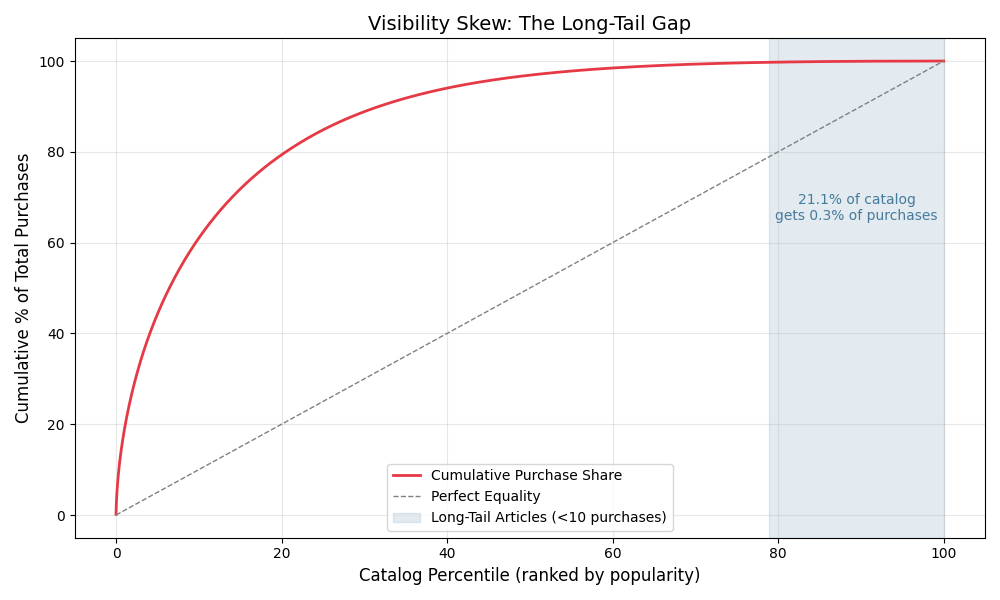
\includegraphics[width=0.75\textwidth]{metrics/EDA_Long_tail_phase1.png}
    \caption{Visibility skew in the H\&M catalog. The vast majority of articles occupy the long tail with minimal transaction volume, while a small fraction of head items dominate.}
    \label{fig:eda_long_tail}
\end{figure}

% ══════════════════════════════════════════════════════════
\section{Methodology}
\label{sec:method}

\subsection{Act 1: The Villain (SASRec + Popularity Bias)}

The Villain is a \textbf{SASRec}-based sequential recommender with an intentionally added popularity amplifier.

\textbf{Embedding layer.}\quad
Item IDs and position indices are mapped to $D{=}128$-dimensional embeddings via learned lookup tables, then summed and layer-normalised:
\begin{equation}
    \mathbf{x} = \text{LayerNorm}\!\left(\mathbf{E}_{\text{item}}[\mathbf{s}] + \mathbf{E}_{\text{pos}}[\mathbf{p}]\right)
\end{equation}
where $\mathbf{s} \in \mathbb{Z}^{B \times S}$ is the padded item sequence and $\mathbf{p}$ the position indices.

\textbf{Transformer encoder.}\quad
A 3-layer causal Transformer encoder with 4 attention heads processes the sequence.
A causal mask ensures each position attends only to itself and earlier positions.

\textbf{Prediction head.}\quad
The hidden state at the last valid position is projected against the item embedding matrix:
\begin{equation}
    \mathbf{z} = \mathbf{h}_{\text{last}} \cdot \mathbf{E}_{\text{item}}^\top \in \mathbb{R}^{V}
\end{equation}

\textbf{Popularity bias.}\quad
A learnable vector $\mathbf{b} \in \mathbb{R}^{V}$ (initialised to ones) multiplies the logits element-wise: $\hat{\mathbf{z}} = \mathbf{z} \odot \mathbf{b}$.
This amplifies scores for popular items.
After training, $\mathbf{b}$ values range from 0.83 to 2.08, confirming the model actively exploits popularity.

\textbf{Training.}\quad
Cross-entropy loss over the full $V{=}26{,}933$ vocabulary, AdamW optimiser (lr$\,{=}\,10^{-3}$, weight decay $0.01$), ReduceLROnPlateau scheduler, batch size 256, early stopping with patience 10.
The model converges in 14 epochs (${\sim}5$ minutes).

The full Villain architecture is shown in \Cref{fig:arch_villain}.

\begin{figure}[H]
    \centering
    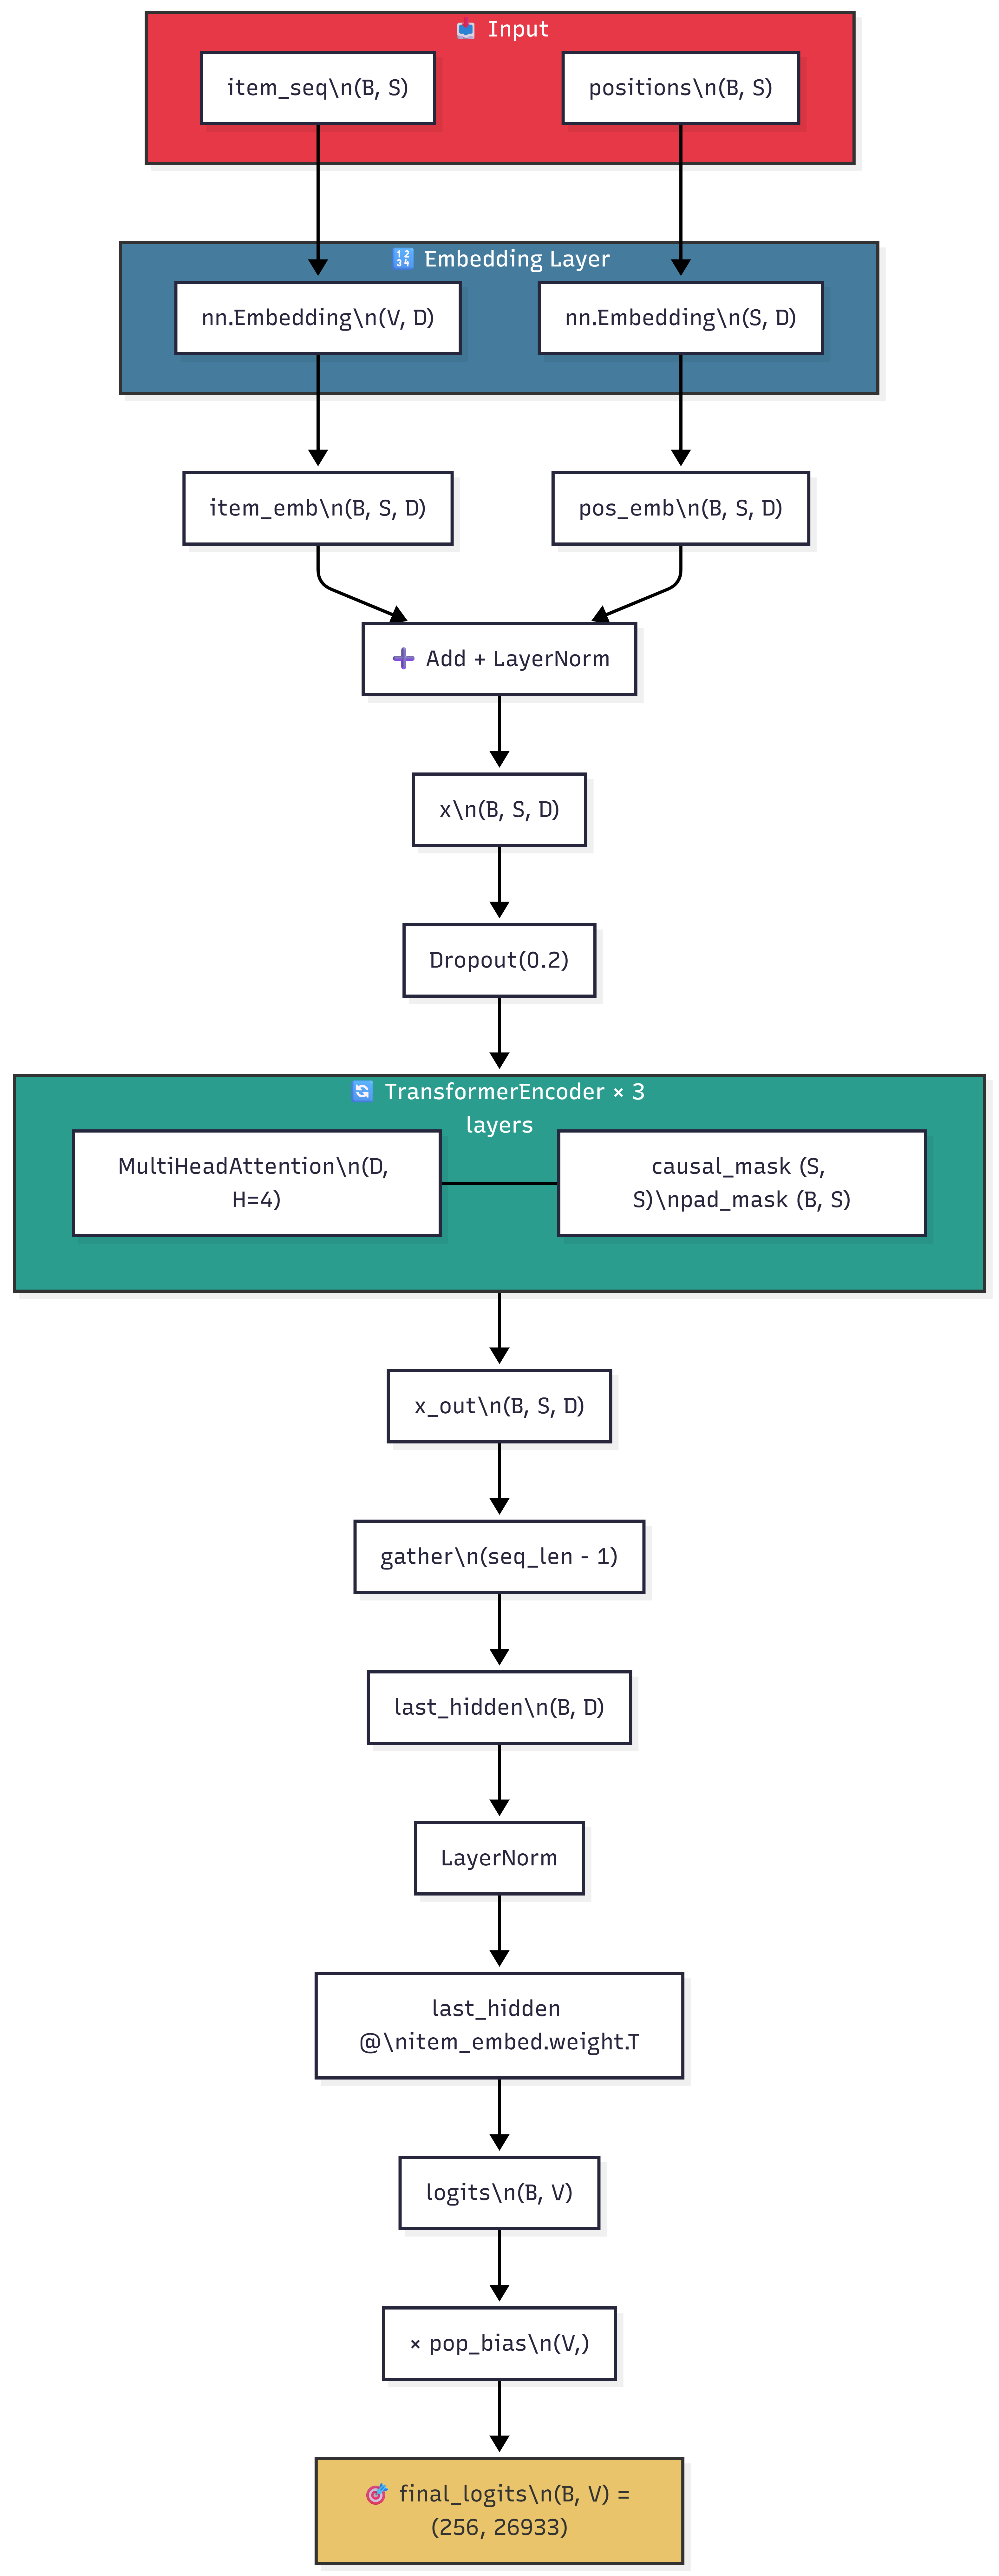
\includegraphics[width=0.82\textwidth]{presentation/mermaid_arch_villain.png.png}
    \caption{Villain architecture: SASRec with learnable popularity bias vector. Input item and position sequences are embedded, summed, and passed through a 3-layer causal Transformer. The output logits are scaled by a learnable popularity bias vector.}
    \label{fig:arch_villain}
\end{figure}

\subsection{Act 2: The Hero (BST + Visual Fusion + Contrastive)}

The Hero extends the Villain with \textbf{multimodal fusion} and \textbf{contrastive learning}.

\textbf{Visual projection.}\quad
For each item in the sequence, the pre-computed 2048-dim ResNet50 embedding is projected to $D{=}128$ via a learnable linear layer, followed by LayerNorm and dropout:
\begin{equation}
    \mathbf{v}_{\text{proj}} = \text{Dropout}\!\left(\text{LayerNorm}\!\left(\mathbf{W}_v \mathbf{v} + \mathbf{b}_v\right)\right)
\end{equation}
where $\mathbf{W}_v \in \mathbb{R}^{D \times 2048}$.

\textbf{Multimodal fusion.}\quad
The projected visual embedding is added element-wise to the ID + position representation before the Transformer encoder:
\begin{equation}
    \mathbf{x}_{\text{fused}} = \text{LayerNorm}\!\left(\mathbf{E}_{\text{item}}[\mathbf{s}] + \mathbf{E}_{\text{pos}}[\mathbf{p}] + \mathbf{v}_{\text{proj}}\right)
\end{equation}

\textbf{Contrastive learning head (InfoNCE).}\quad
The final hidden state serves as an \emph{anchor}; the target item's embedding is the \emph{positive}; and $N{=}10$ hard negatives are mined via attribute-aware Jaccard similarity (see \S\ref{sec:hardneg}).
The InfoNCE loss is:
\begin{equation}
\mathcal{L}_{\text{InfoNCE}} = -\log \frac{
    \exp\!\big(\text{sim}(\mathbf{a}, \mathbf{p}^+)\,/\,\tau\big)
}{
    \exp\!\big(\text{sim}(\mathbf{a}, \mathbf{p}^+)\,/\,\tau\big)
    + {\displaystyle\sum_{j}}\,\exp\!\big(\text{sim}(\mathbf{a}, \mathbf{n}_j)\,/\,\tau\big)
}
\end{equation}
with temperature $\tau{=}0.07$.

\textbf{Combined loss.}
\begin{equation}
    \mathcal{L}_{\text{Hero}} = \mathcal{L}_{\text{CE}} + \lambda_{\text{CL}} \cdot \mathcal{L}_{\text{InfoNCE}}, \quad \lambda_{\text{CL}} = 0.3
\end{equation}

\textbf{Training.}\quad
AdamW (lr$\,{=}\,5{\times}10^{-4}$, weight decay $0.01$), batch size 128, 50 epochs, early stopping with patience 10.
Dropout is reduced to 0.1 to avoid underfitting on the richer input signal.

The full Hero architecture is shown in \Cref{fig:arch_hero}.

\begin{figure}[H]
    \centering
    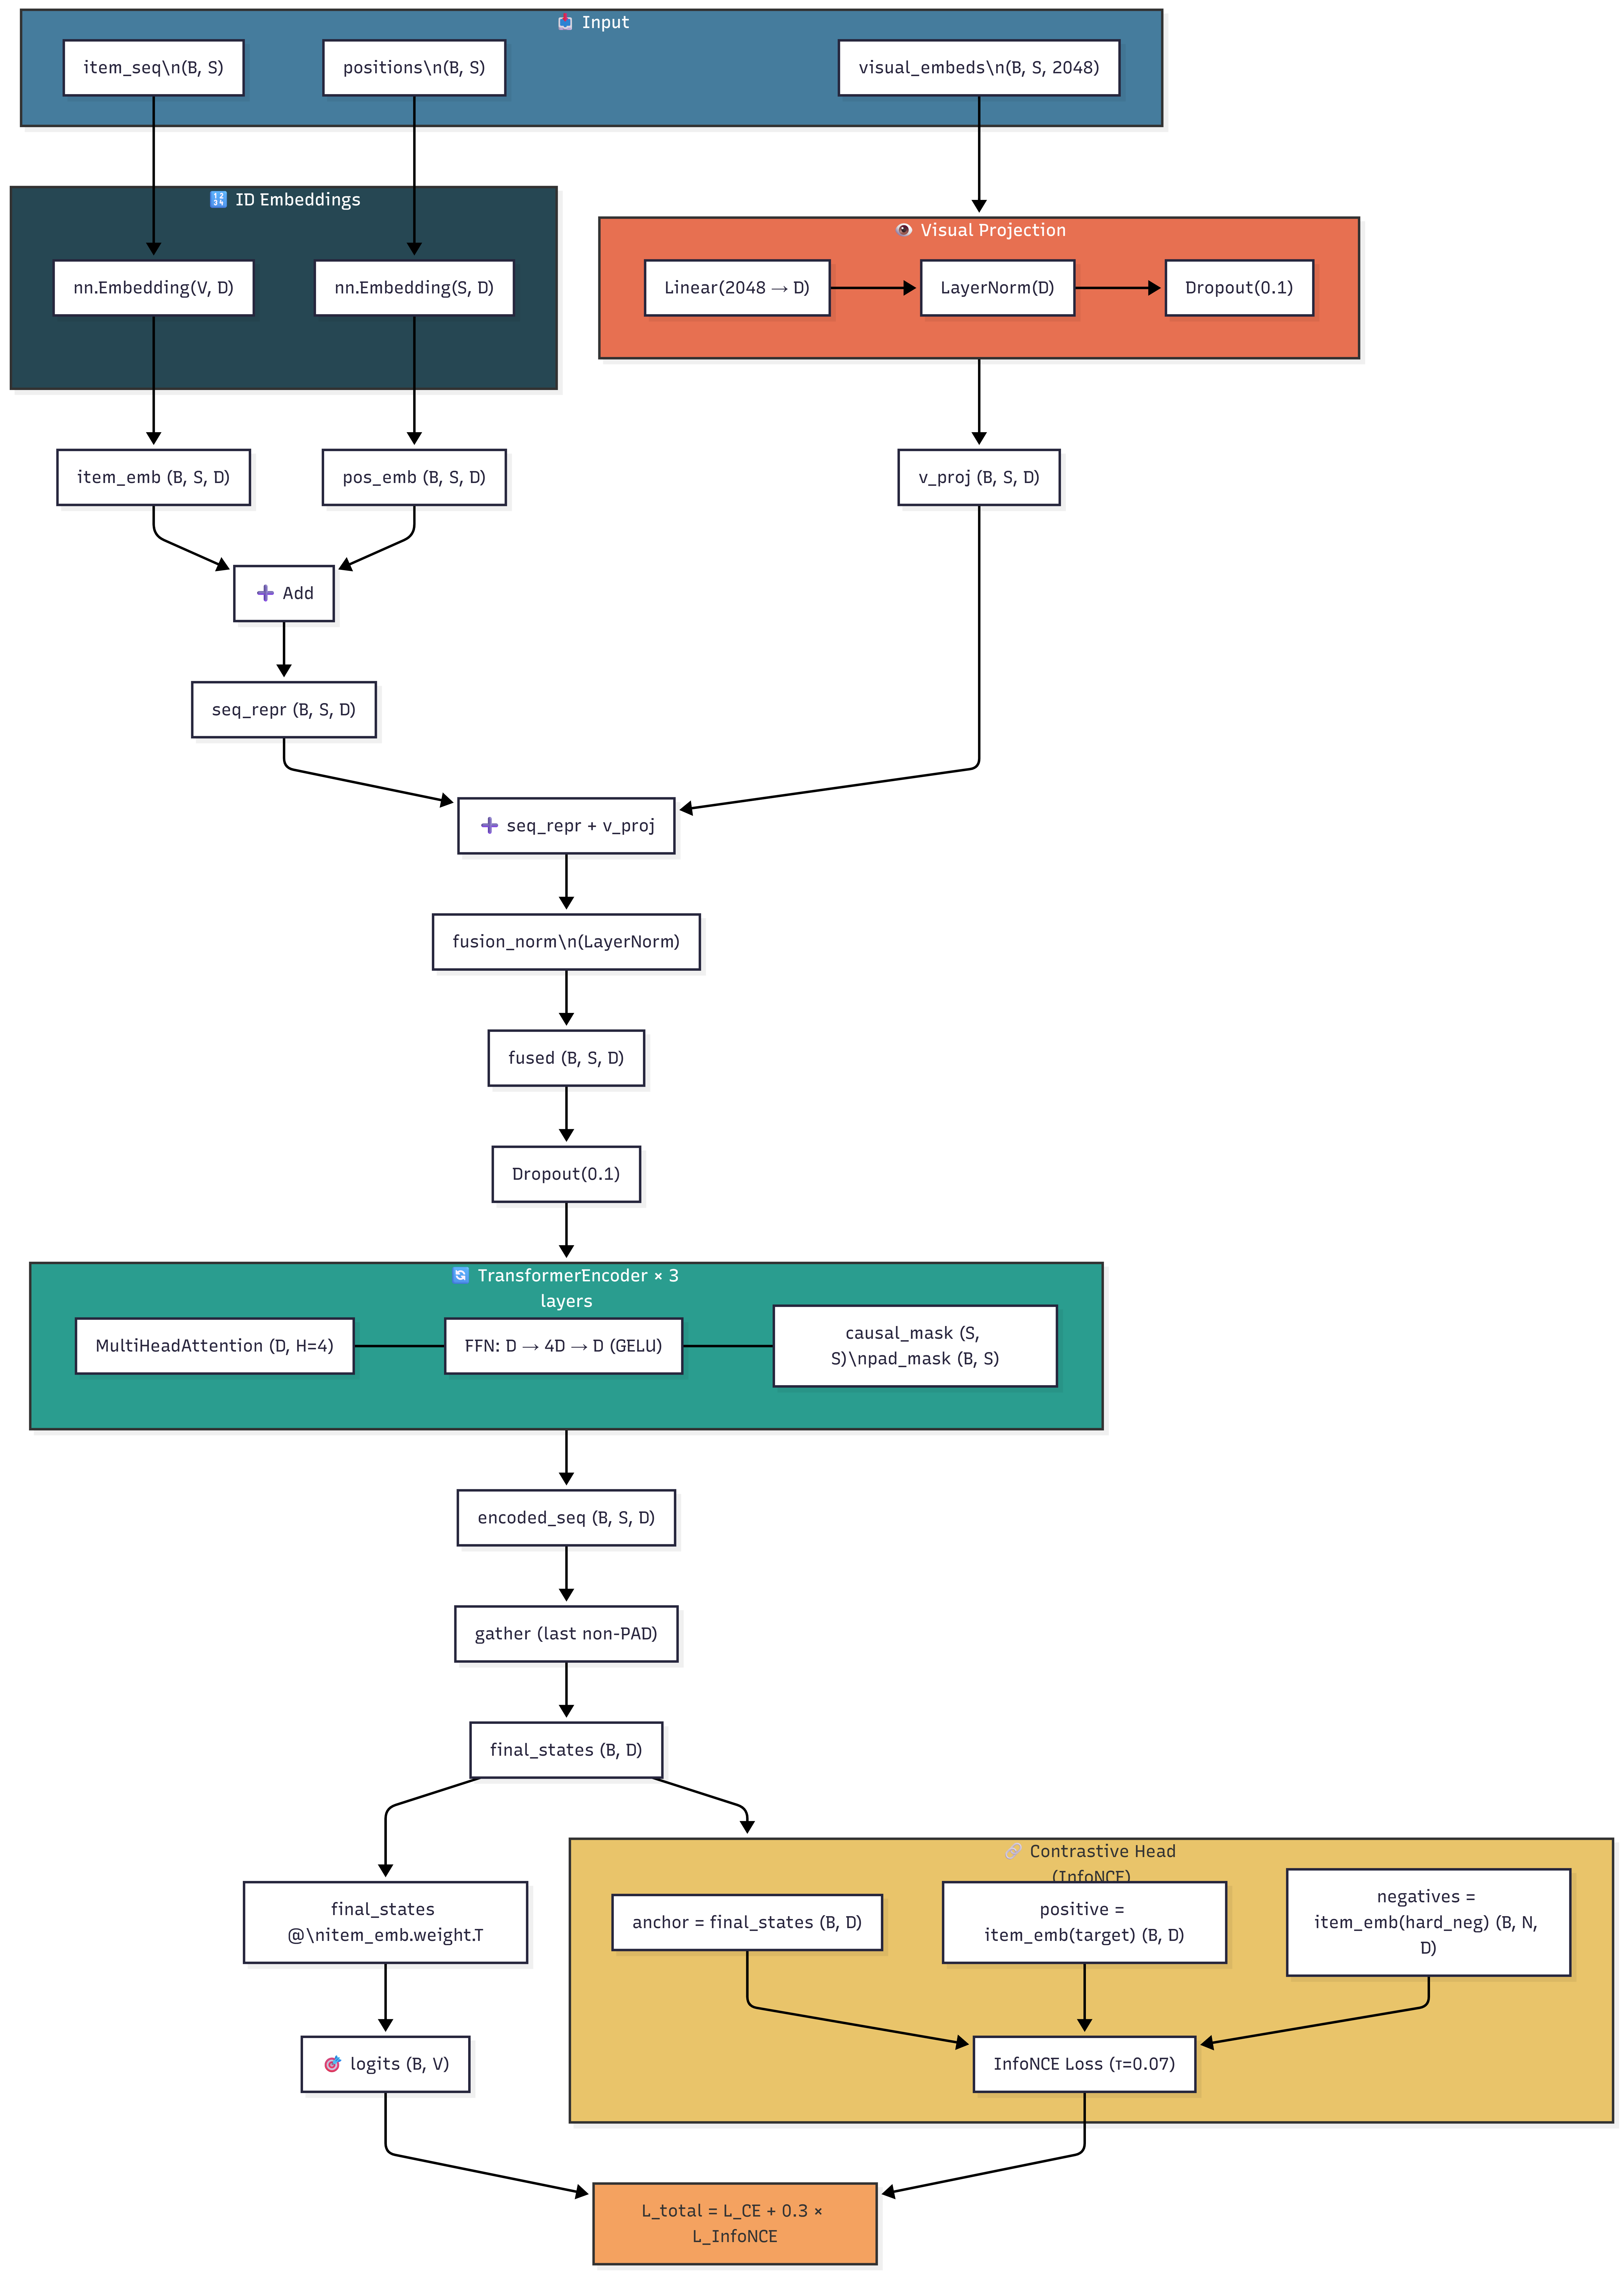
\includegraphics[width=0.85\textwidth]{presentation/mermaid_arch_hero.png.png}
    \caption{Hero architecture: Behavior Sequence Transformer with ResNet50 visual fusion and InfoNCE contrastive learning head.}
    \label{fig:arch_hero}
\end{figure}

\subsubsection{Attribute-Aware Hard-Negative Mining}
\label{sec:hardneg}

Random negative sampling produces trivially dissimilar items (e.g., a shoe vs.\ a hat), yielding weak contrastive gradients.
We replace this with \textbf{Jaccard-based attribute-aware mining}: for each item, we compute the pairwise Jaccard similarity over binarised attributes (\texttt{product\_group}, \texttt{colour\_group}, \texttt{garment\_group}) and select $N{=}10$ negatives with Jaccard $\in [0.3, 0.7]$ --- items that share \emph{some} but not \emph{all} properties.

The full pairwise computation is $O(V^2)$, mitigated by chunked processing (512-row chunks) to cap peak memory.
The resulting $(V, N)$ index matrix is cached to disk (${\sim}6.3$s to compute, instant reload).

\subsection{Act 3: The Brain (Multi-Objective Discovery Loss)}

To explicitly control the trade-off between ranking accuracy and catalog exploration, we extend the Hero loss to a \textbf{three-term objective}:
\begin{equation}
    \mathcal{L}_{\text{total}} = \mathcal{L}_{\text{CE}} + \lambda_{\text{CL}} \cdot \mathcal{L}_{\text{InfoNCE}} + \lambda_{\text{disc}} \cdot \mathcal{L}_{\text{disc}}
    \label{eq:total_loss}
\end{equation}

\textbf{Discovery loss.}\quad
The discovery term penalises placing high softmax mass on popular items:
\begin{equation}
    \mathcal{L}_{\text{disc}} = \frac{1}{B}\sum_{i=1}^{B} \text{softmax}(\mathbf{z}_i)^\top \cdot \mathbf{q}
\end{equation}
where $\mathbf{q} \in \mathbb{R}^{V}$ is a pre-computed popularity logit vector (log-smoothed transaction counts).
Using soft (softmax-weighted) scores keeps gradients smooth; setting $\lambda_{\text{disc}}{=}0$ exactly recovers Phase~2 behaviour.

\textbf{Pareto sweep.}\quad
We fine-tune the Phase~2 Hero checkpoint for 20 epochs at each $\lambda_{\text{disc}} \in \{0.0, 0.3, 0.7, 1.0\}$, using a fresh AdamW optimiser per sweep point to avoid momentum contamination.

The architecture for the discovery loss extension is shown in \Cref{fig:arch_discovery}.

\begin{figure}[H]
    \centering
    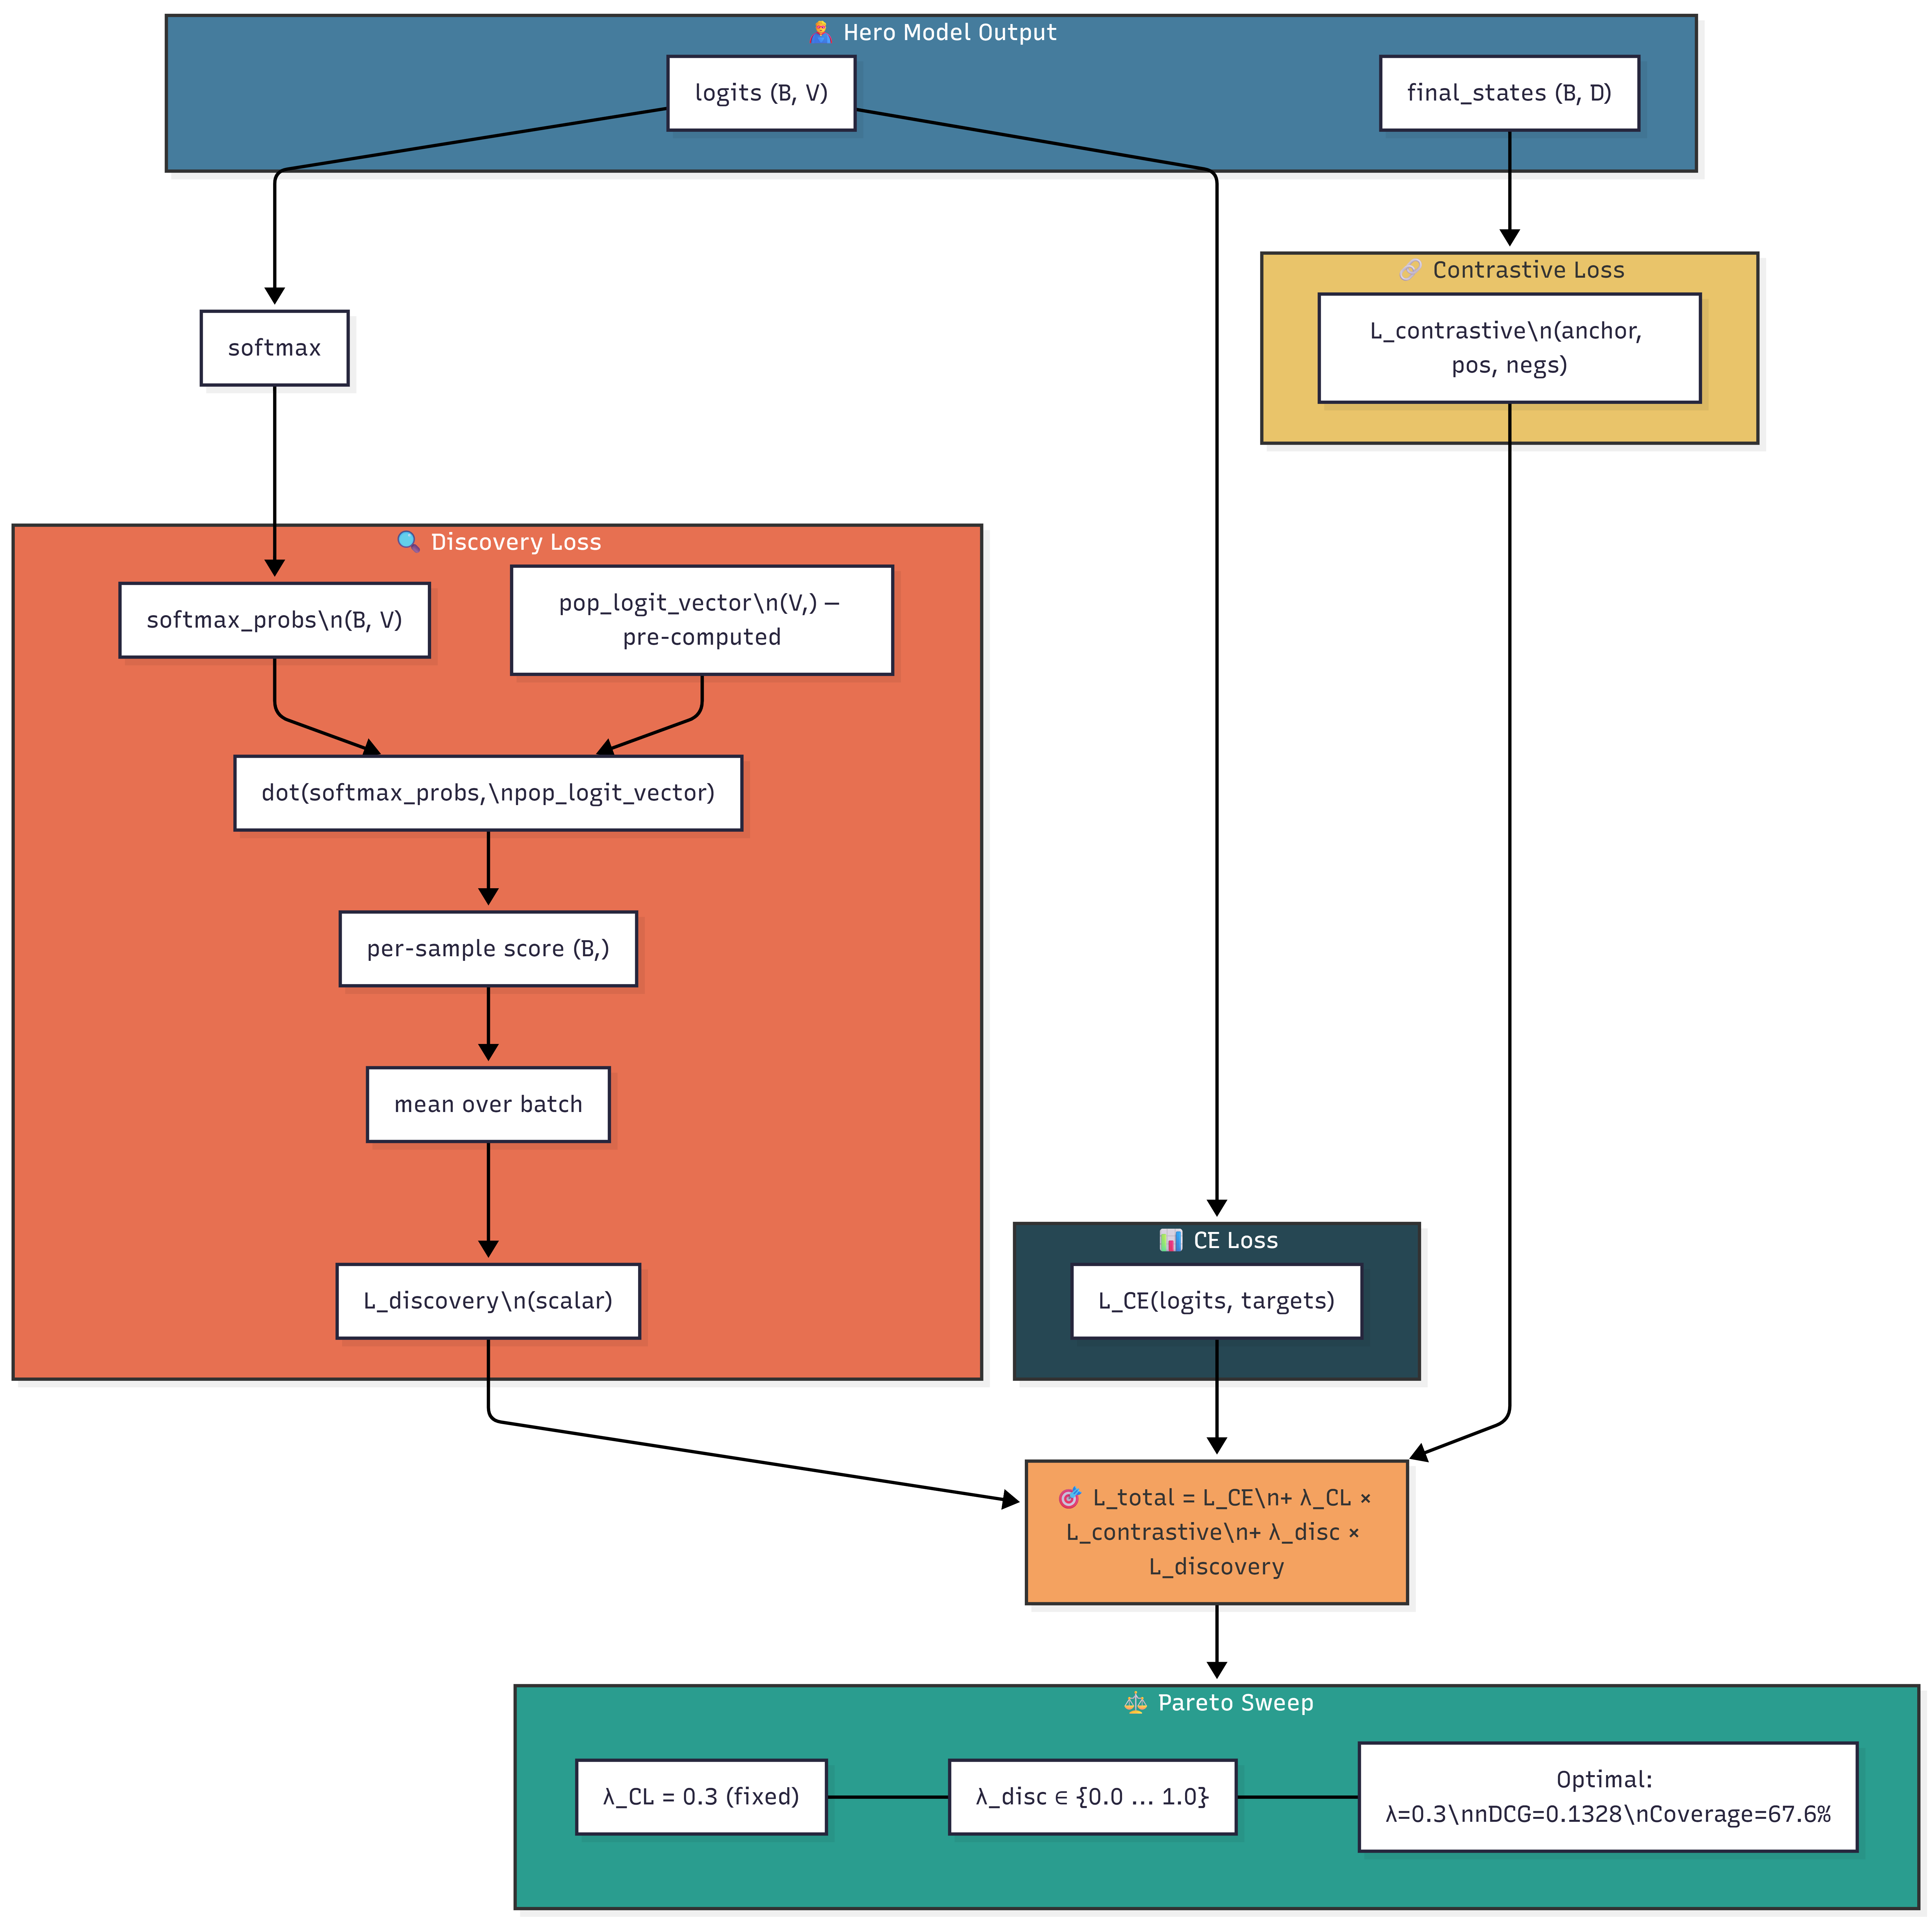
\includegraphics[width=0.85\textwidth]{presentation/mermaid_arch_discovery_loss.png.png}
    \caption{Discovery loss extension: differentiable penalty on softmax mass over popular items, integrated into the three-term multi-objective loss with tuneable $\lambda_{\text{disc}}$.}
    \label{fig:arch_discovery}
\end{figure}

% ══════════════════════════════════════════════════════════
\section{Evaluation Metrics}
\label{sec:metrics}

We evaluate all models on a multi-objective metric suite:
\begin{itemize}[leftmargin=*,itemsep=2pt]
    \item \textbf{nDCG@12} --- Normalised Discounted Cumulative Gain at rank 12, measuring ranking quality.
    \item \textbf{MRR} --- Mean Reciprocal Rank of the first relevant item.
    \item \textbf{Catalog Coverage} --- fraction of the full catalog appearing in any user's top-12 recommendations.
    \item \textbf{Tail-Item Rate} --- fraction of all top-12 recommendations that are long-tail items ($<\!10$ purchases).
\end{itemize}

% ══════════════════════════════════════════════════════════
\section{Results}
\label{sec:results}

\subsection{Villain vs.\ Hero}

\Cref{tab:main_results} presents the headline comparison.
The Villain achieves the highest nDCG@12 (0.145) but at the cost of extreme popularity bias: 76.3\% of its recommendations go to head items and only 2.2\% to tail items.
The Hero sacrifices 9\% relative nDCG but improves catalog coverage by $+4.2$~pp and nearly doubles the tail-item rate to 4.2\%.

\begin{table}[H]
\centering
\caption{Main results comparing Villain, Hero, and Pareto-optimal Hero ($\lambda_{\text{disc}}{=}0.3$).}
\label{tab:main_results}
\vspace{4pt}
\begin{tabular}{@{}lcccc@{}}
\toprule
\textbf{Model} & \textbf{nDCG@12} & \textbf{MRR} & \textbf{Coverage} & \textbf{Tail Rate} \\
\midrule
Villain          & 0.145 & 0.132 & 57.8\% & 2.2\% \\
Hero ($\lambda{=}0$)    & 0.132 & 0.121 & 60.0\% & 4.2\% \\
Hero ($\lambda{=}0.3$)  & \textbf{0.133} & \textbf{0.123} & \textbf{67.6\%} & \textbf{6.6\%} \\
Hero ($\lambda{=}0.7$)  & 0.085 & 0.073 & 74.6\% & 81.7\% \\
Hero ($\lambda{=}1.0$)  & 0.065 & 0.052 & 71.5\% & 88.2\% \\
\bottomrule
\end{tabular}
\end{table}

\begin{figure}[H]
    \centering
    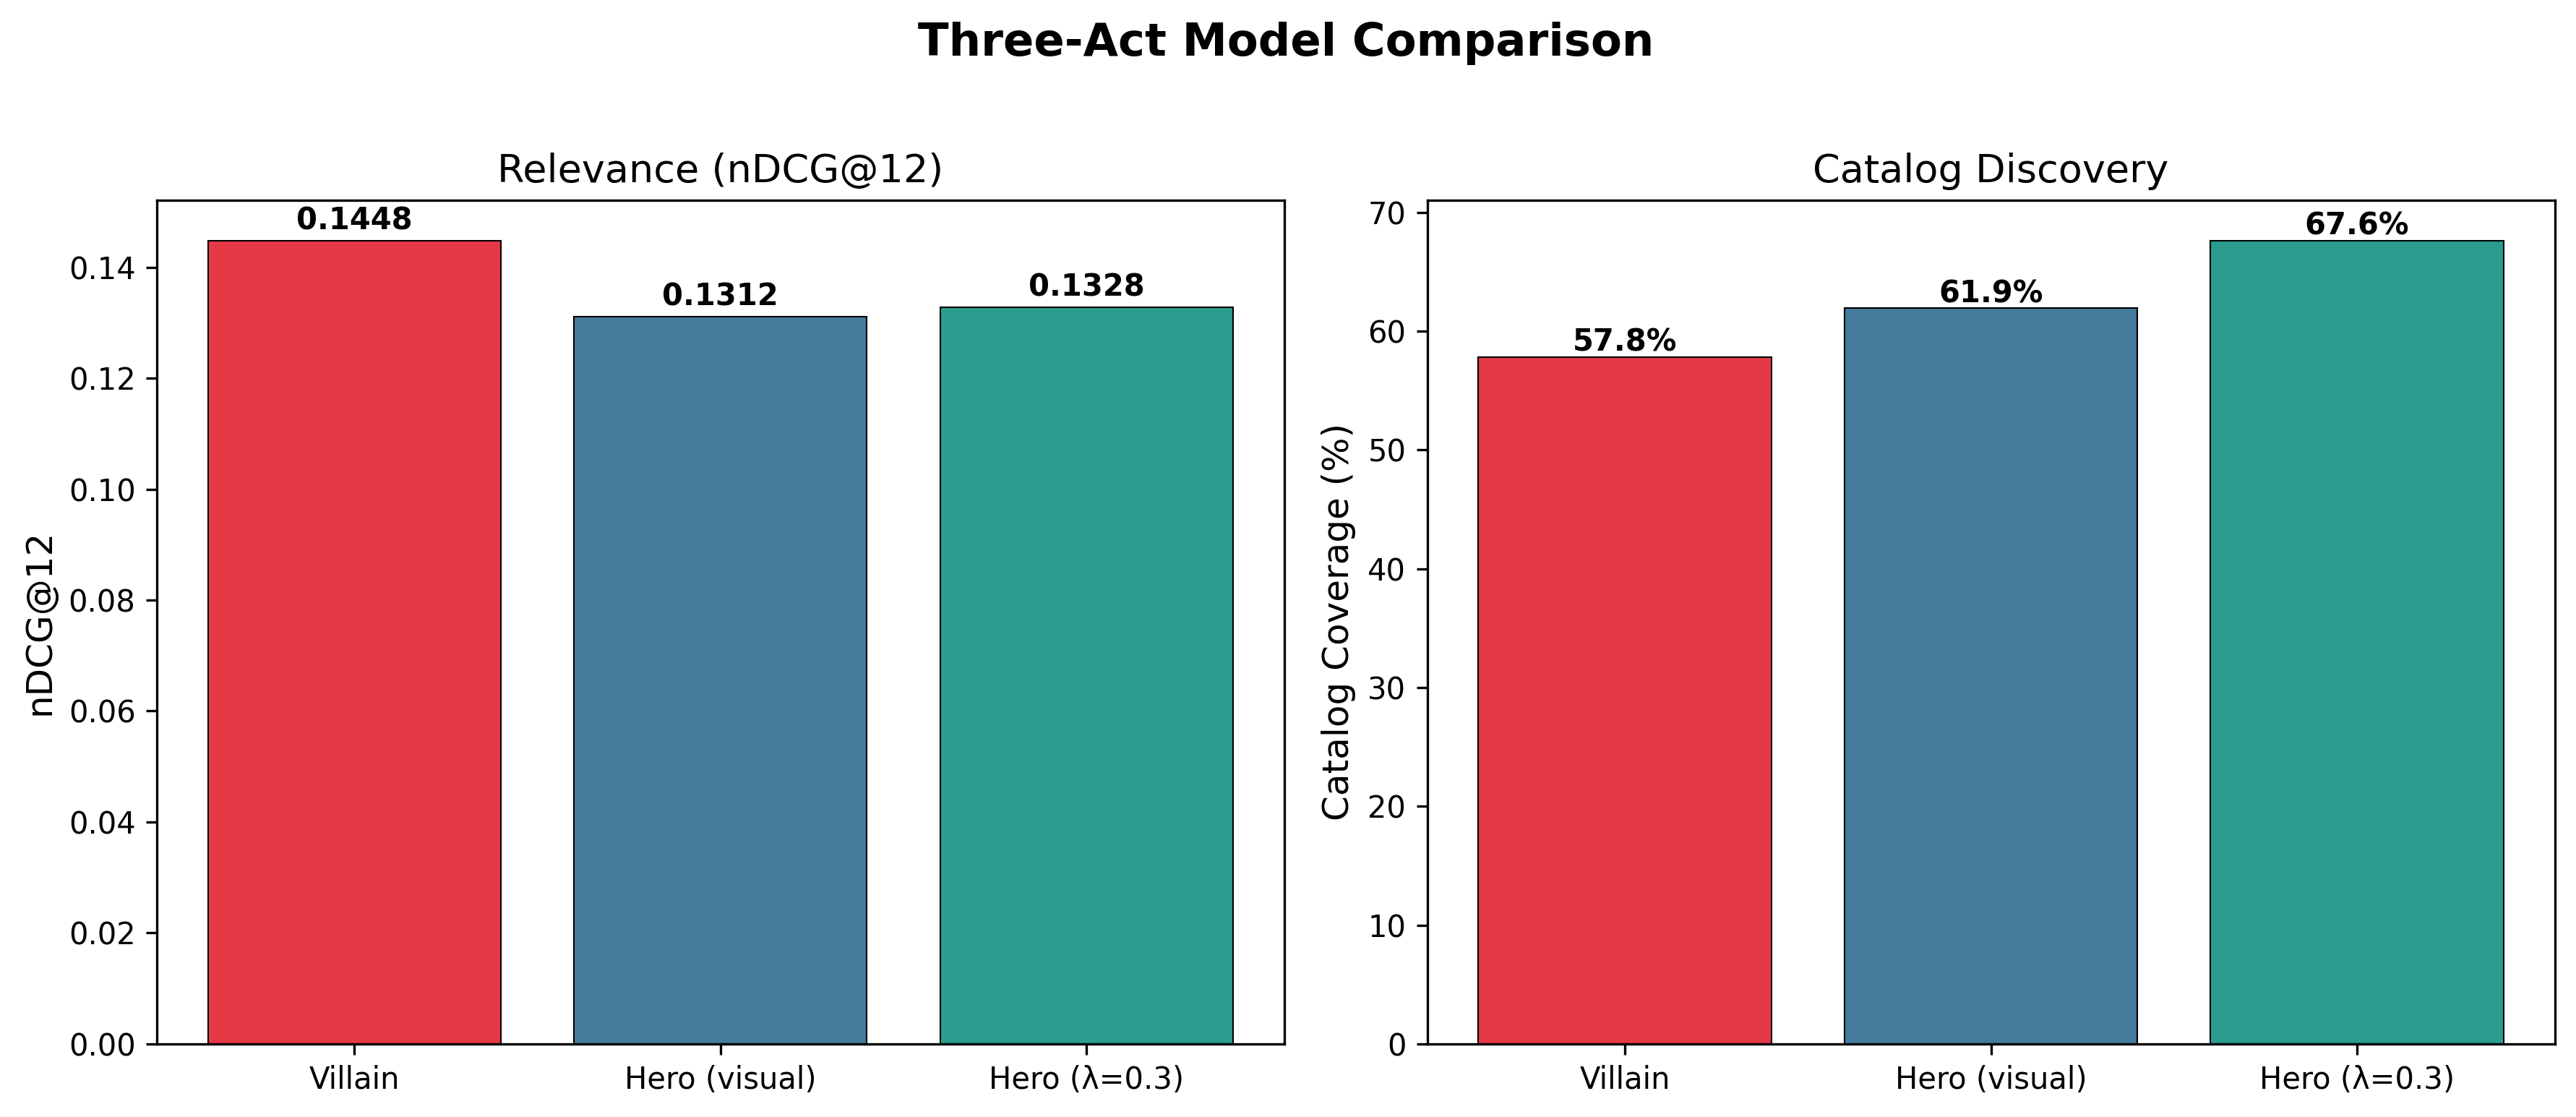
\includegraphics[width=0.78\textwidth]{presentation/model_comparison.png}
    \caption{Side-by-side nDCG@12 and catalog coverage comparison across Villain, Hero, and Pareto-optimal Hero.}
    \label{fig:model_comparison}
\end{figure}

\subsection{Training Dynamics}

\Cref{fig:training_curves} shows the training loss and validation nDCG@12 convergence for both models.
The Villain converges rapidly (14 epochs, ${\sim}5$ min) due to its simpler text-only architecture.
The Hero trains for 44 epochs (${\sim}28$ min) with a gentler convergence curve, reflecting the richer multimodal input and contrastive objective.

\begin{figure}[H]
    \centering
    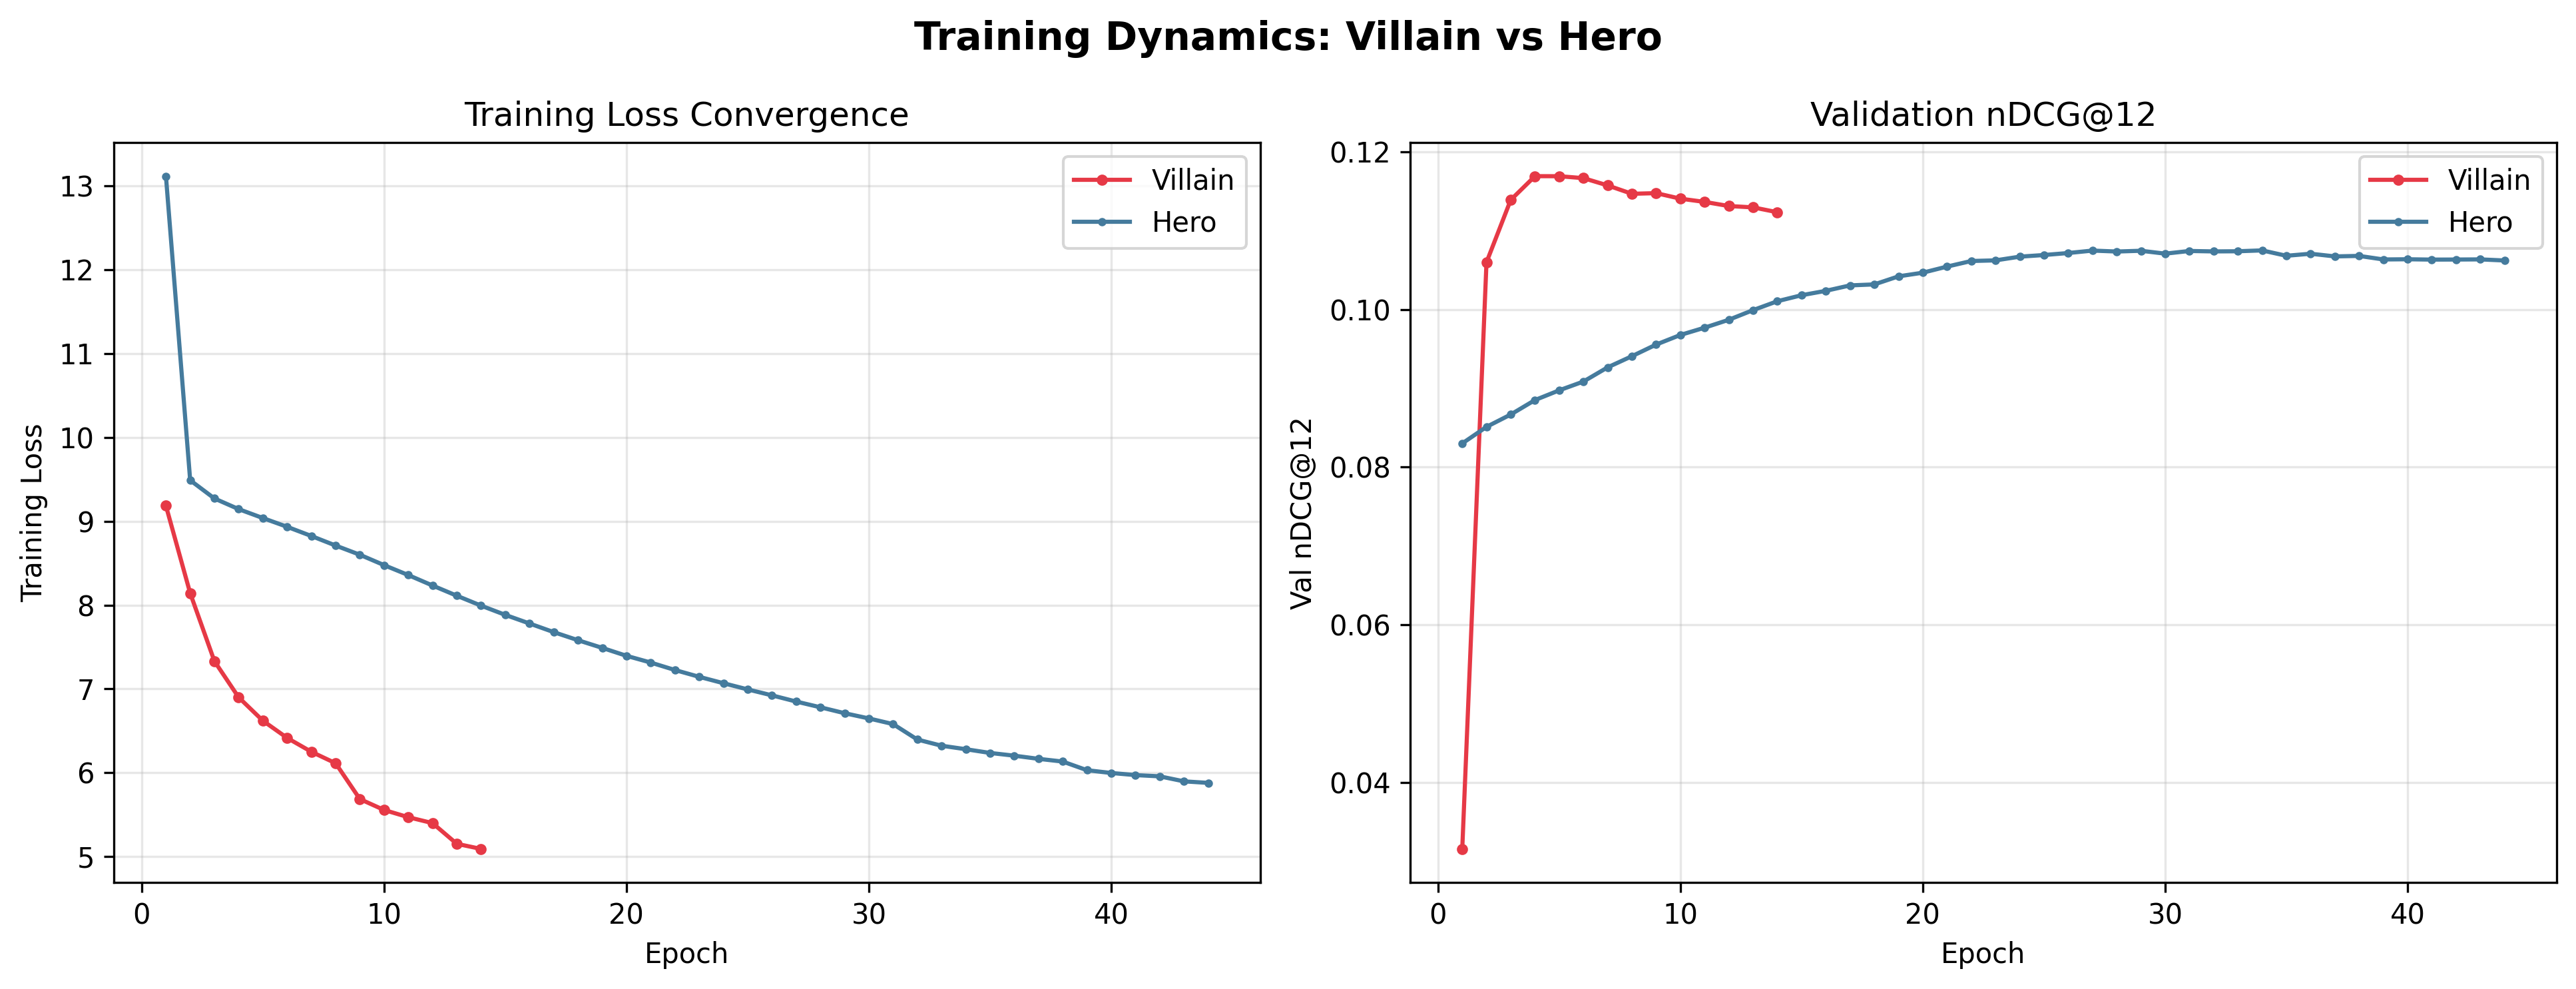
\includegraphics[width=0.78\textwidth]{presentation/training_curves.png}
    \caption{Training loss and validation nDCG@12 for the Villain and Hero models.}
    \label{fig:training_curves}
\end{figure}

\subsection{Multi-Objective Pareto Analysis}

\Cref{fig:pareto_front} shows the Pareto front in the nDCG@12 vs.\ catalog coverage space.
The key findings are:
\begin{itemize}[leftmargin=*,itemsep=2pt]
    \item \textbf{$\lambda{=}0.3$ is Pareto-optimal}: coverage jumps $+7.6$~pp (60.0\%$\to$67.6\%) with \emph{no} nDCG sacrifice (0.132$\to$0.133).
    \item At $\lambda{=}0.7$, coverage reaches 74.6\% but nDCG drops to 0.085 --- an unacceptable accuracy loss.
    \item $\lambda{=}1.0$ actually \emph{reduces} coverage (71.5\%) compared to $\lambda{=}0.7$, suggesting the model collapses when discovery pressure is too high.
\end{itemize}

\begin{figure}[H]
    \centering
    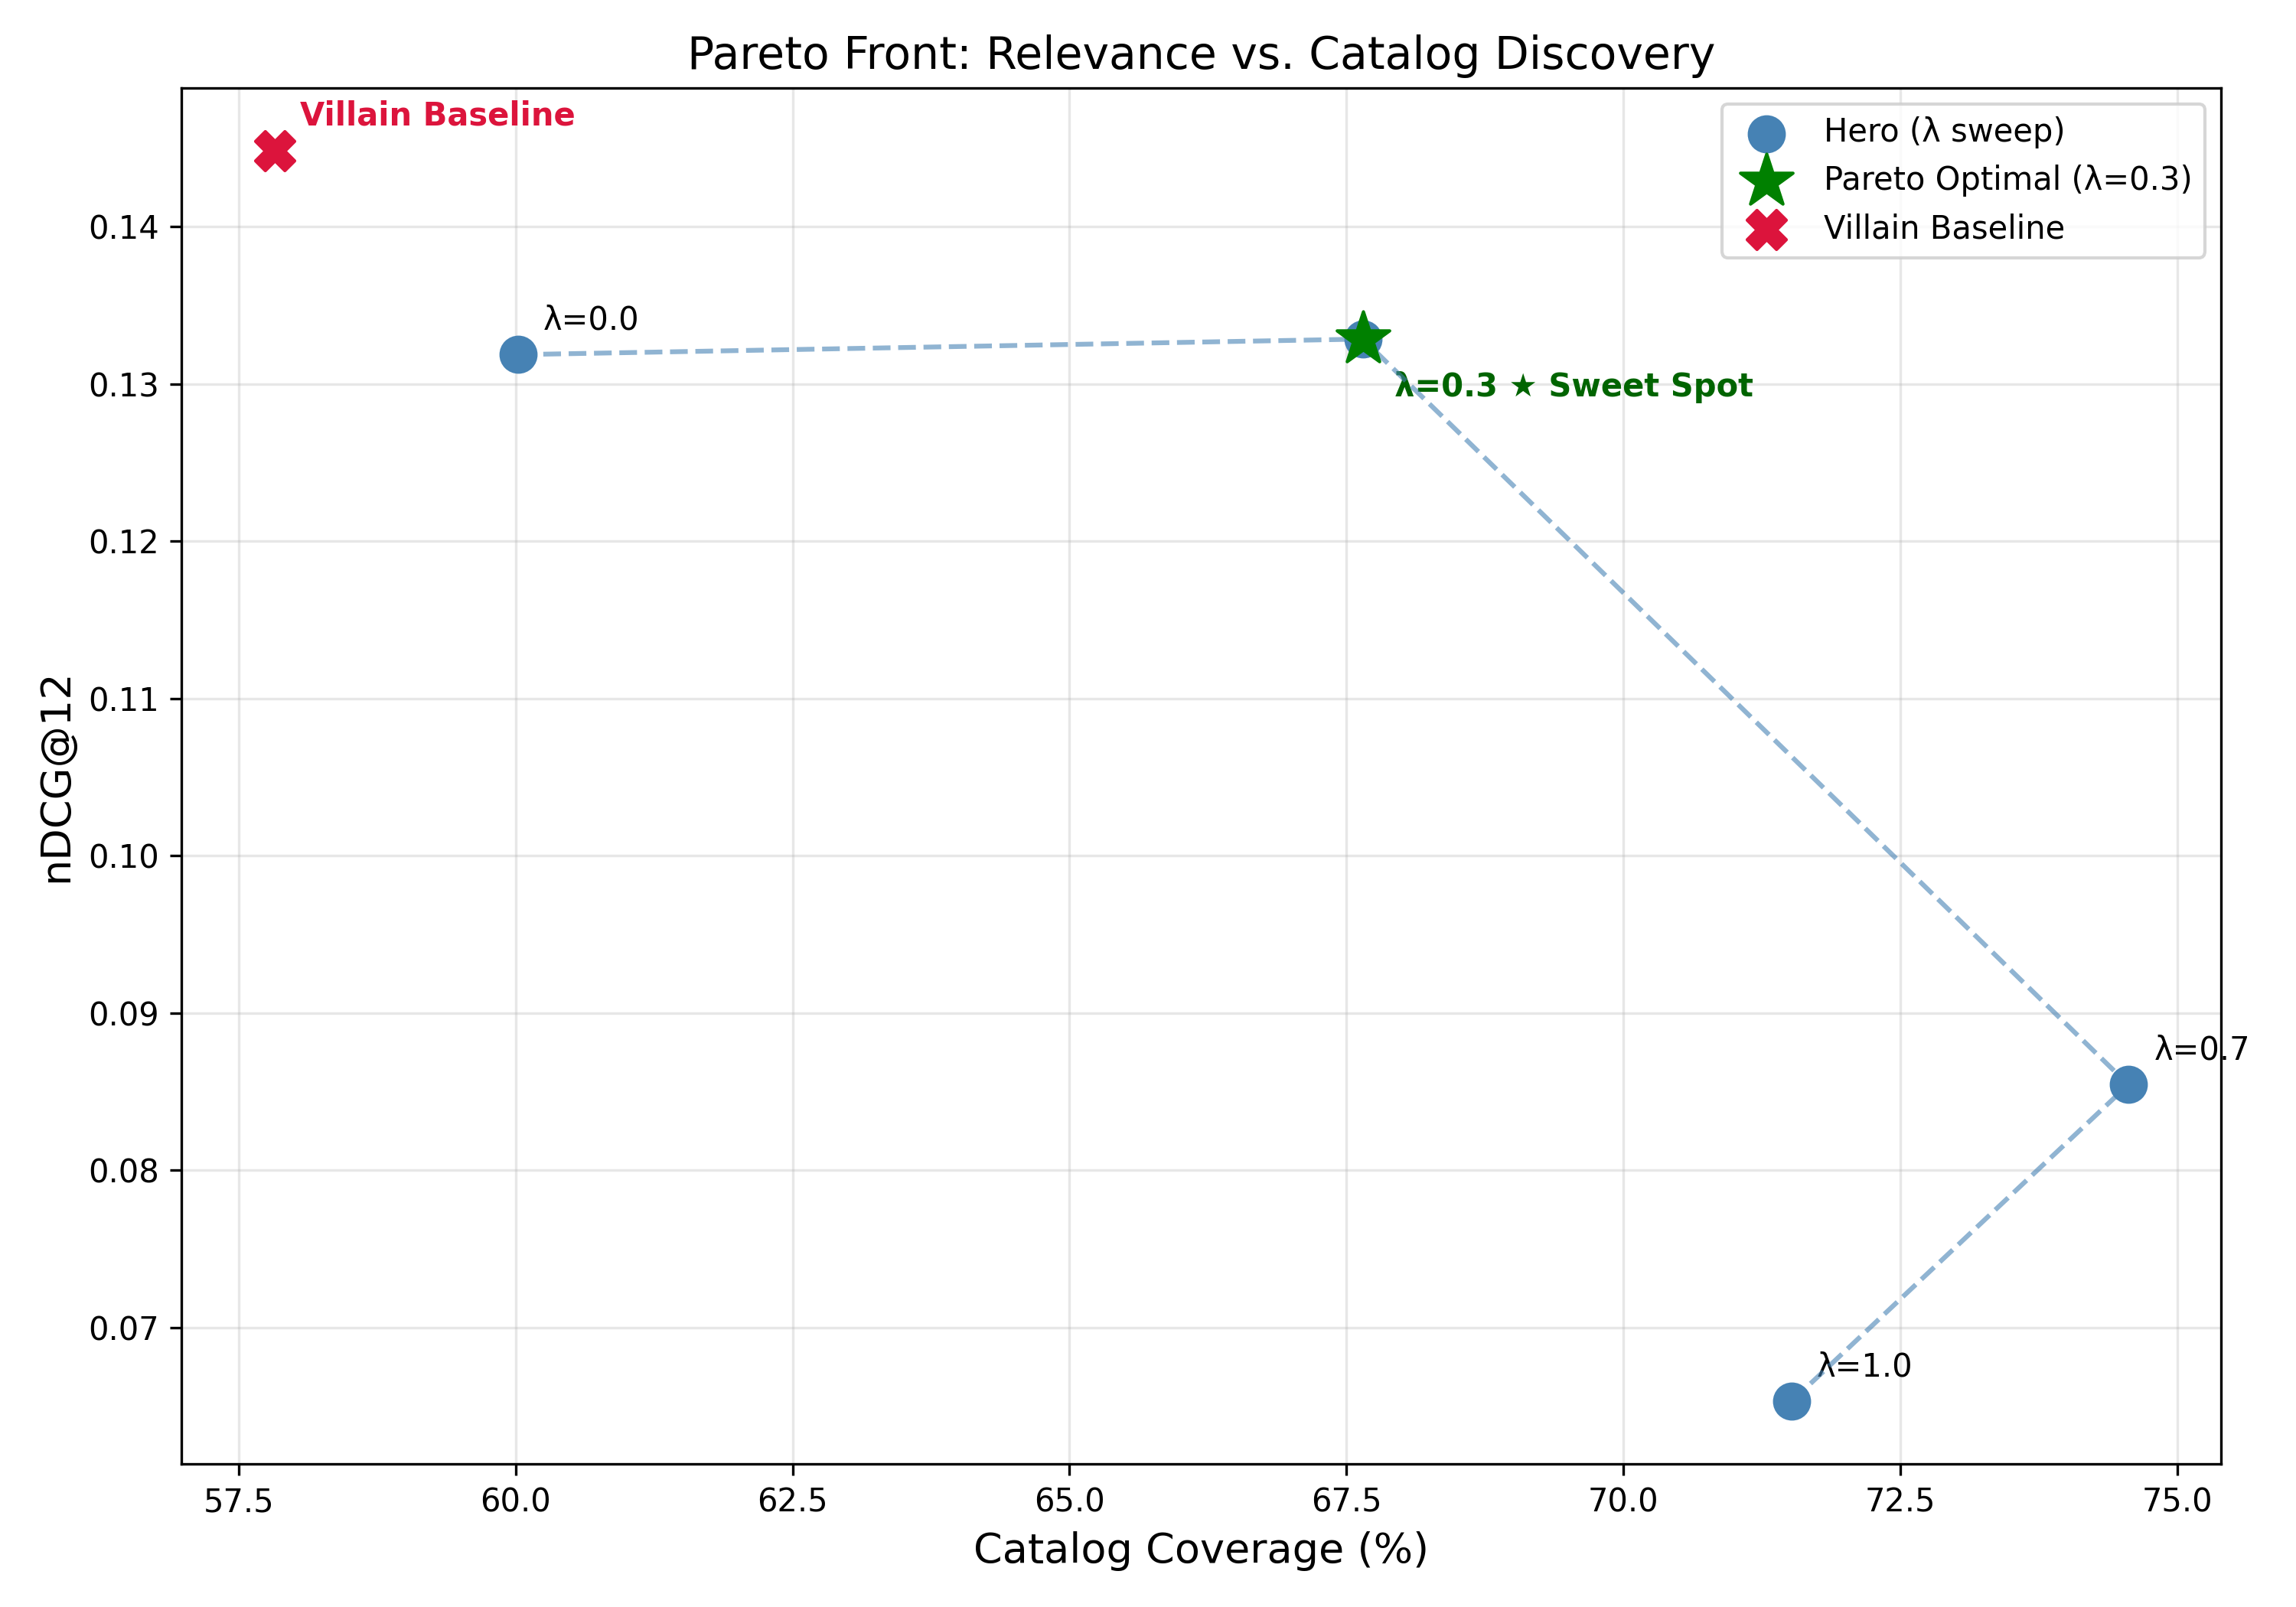
\includegraphics[width=0.78\textwidth]{pareto/pareto_front.png}
    \caption{Pareto front: nDCG@12 vs.\ catalog coverage for different $\lambda_{\text{disc}}$ values. The Villain baseline is overlaid. $\lambda{=}0.3$ dominates.}
    \label{fig:pareto_front}
\end{figure}

\Cref{fig:tail_rate_curve} shows the tail-item rate as a function of $\lambda_{\text{disc}}$.
At $\lambda{=}0.3$, the tail-item rate rises to 6.6\% (3$\times$ the Villain's 2.2\%).
Beyond $\lambda{=}0.7$, the model over-corrects, pushing $>80\%$ of recommendations to tail items.

\begin{figure}[H]
    \centering
    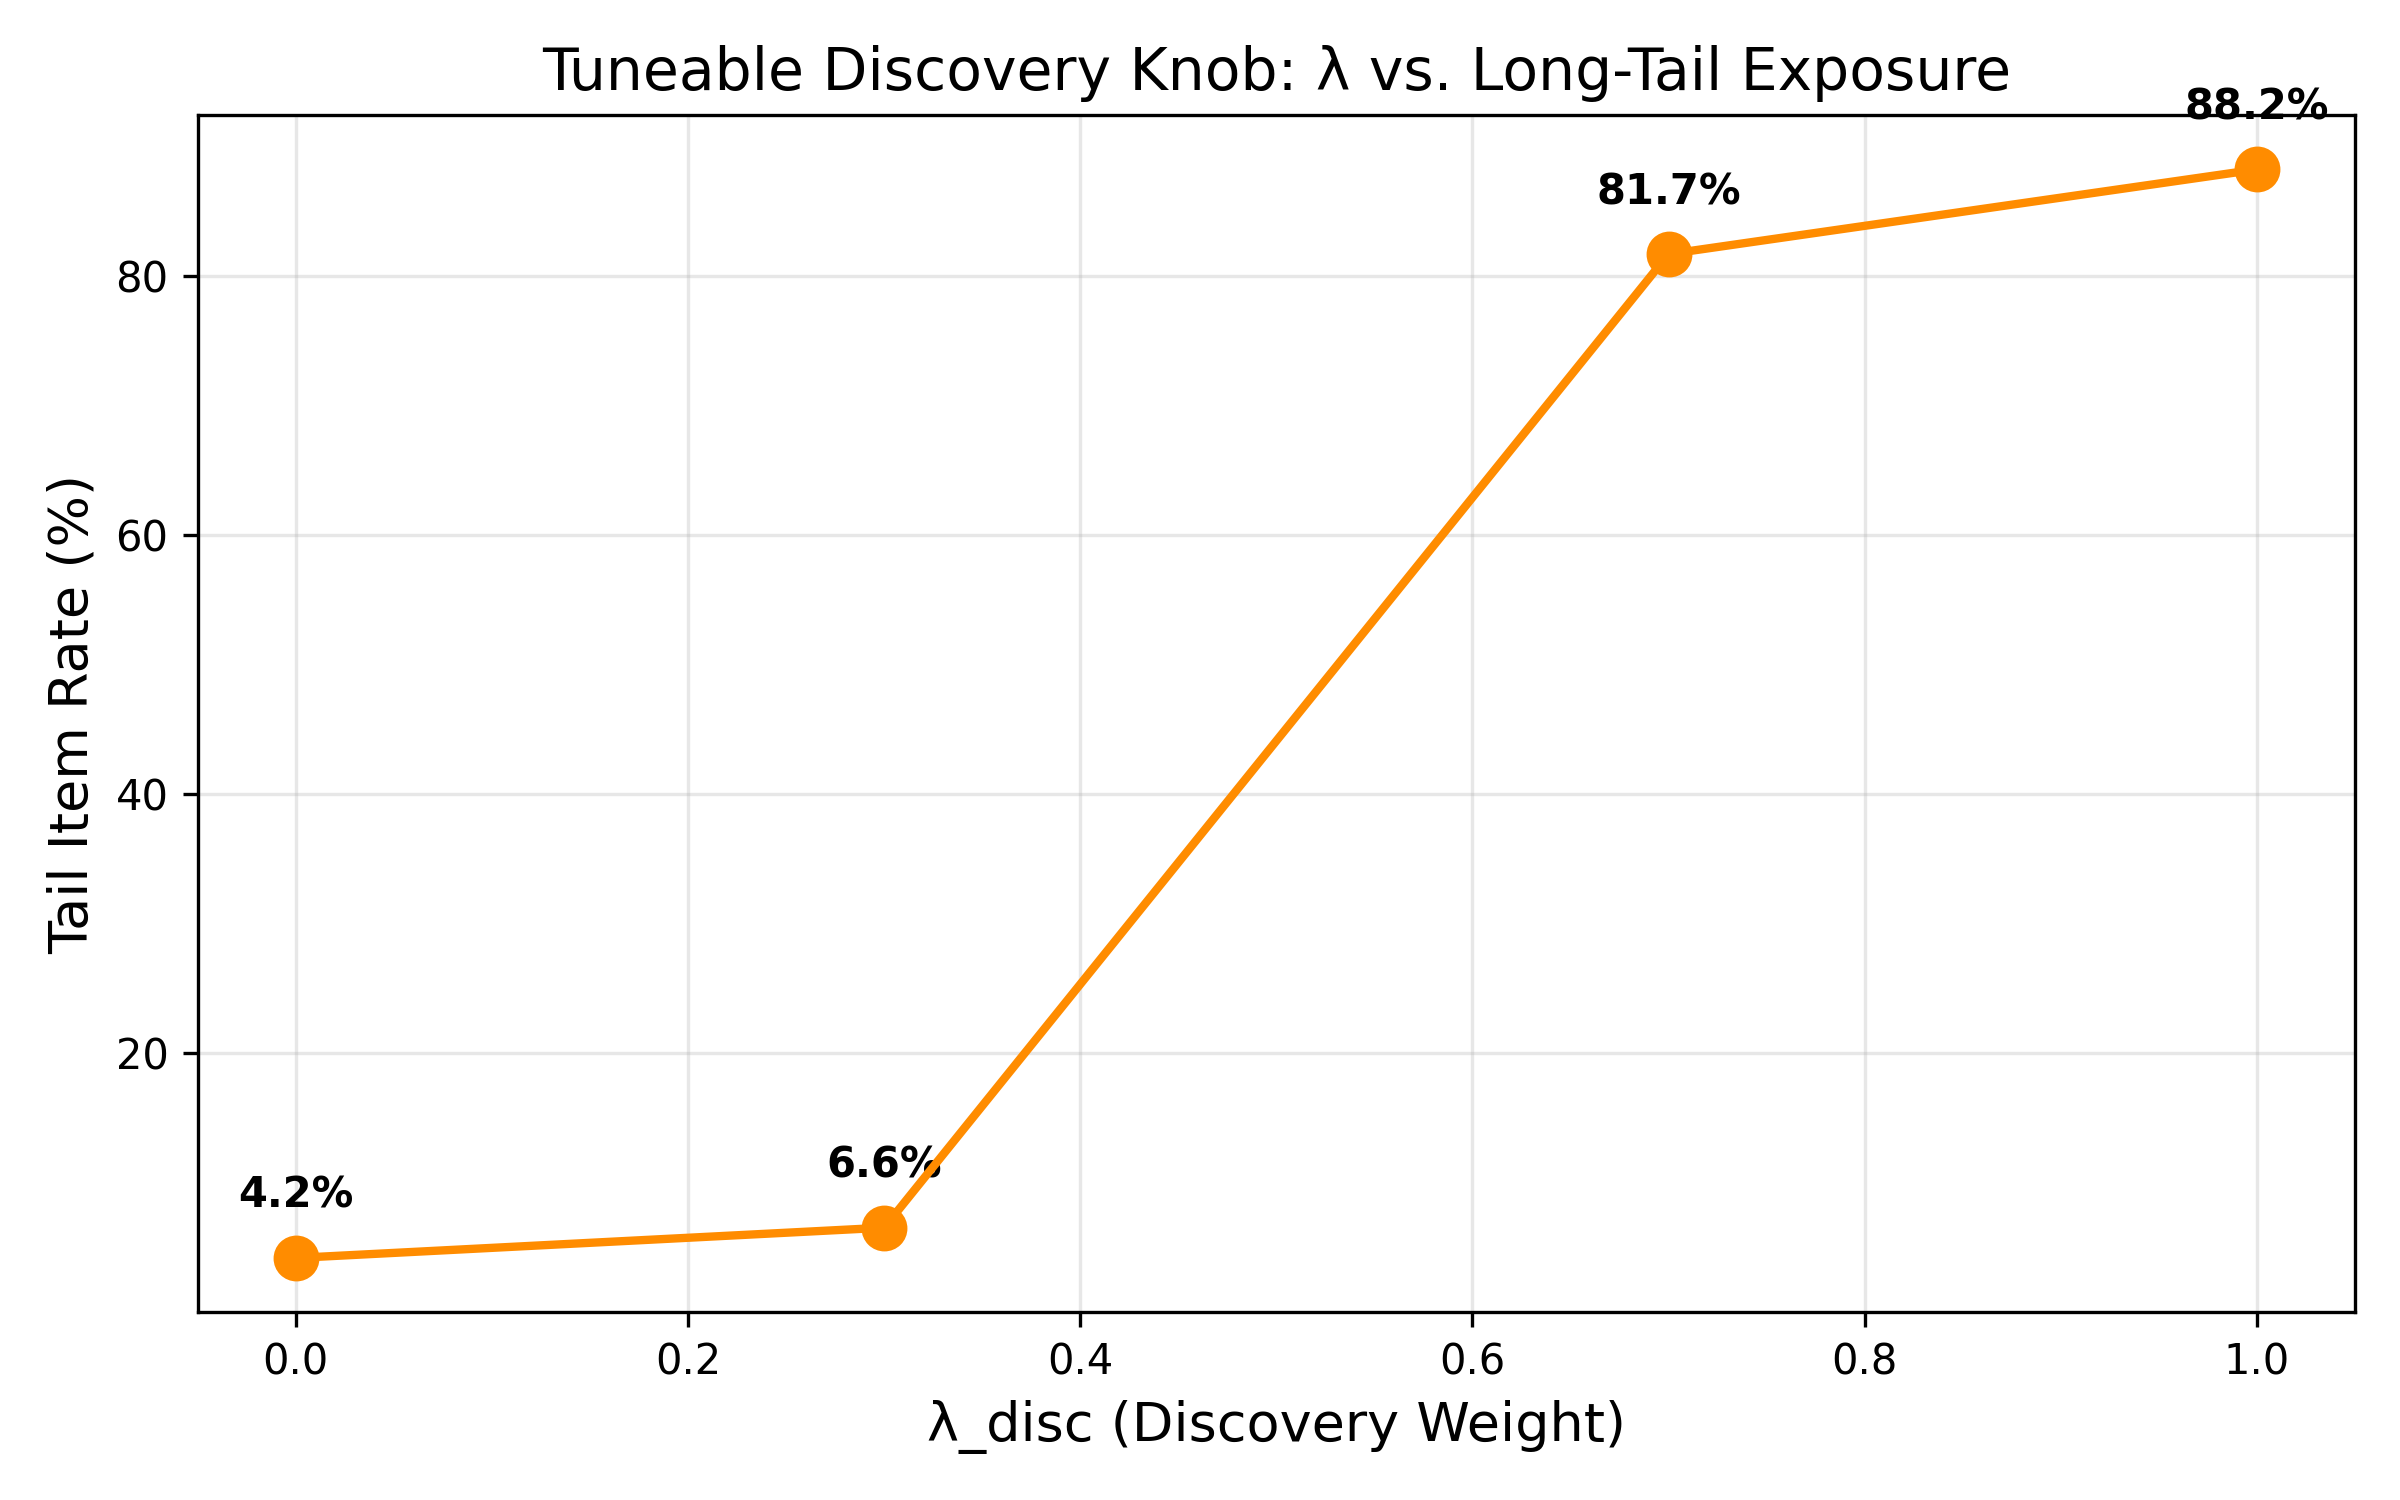
\includegraphics[width=0.78\textwidth]{pareto/tail_rate_curve.png}
    \caption{Tail-item recommendation rate as a function of discovery loss weight $\lambda_{\text{disc}}$.}
    \label{fig:tail_rate_curve}
\end{figure}

\subsection{Visual Ablation Study}

To isolate the contribution of visual features, we train an \textbf{ID-only Hero} (identical architecture minus the \texttt{VisualProjection} module) from scratch with the same hyperparameters.
Results are shown in \Cref{tab:ablation} and \Cref{fig:ablation}.

\begin{table}[H]
\centering
\caption{Visual ablation: ID-only Hero vs.\ full Hero with ResNet50 embeddings.}
\label{tab:ablation}
\vspace{4pt}
\begin{tabular}{@{}lccc@{}}
\toprule
\textbf{Model} & \textbf{nDCG@12} & \textbf{Coverage} & \textbf{Cold-Start Rank} \\
\midrule
Villain          & 0.145 & 57.8\% & 26{,}159 \\
Hero (ID-only)   & 0.131 & 60.7\% & 24{,}900 \\
Hero (visual)    & 0.131 & 61.9\% & 20{,}375 \\
\midrule
\textbf{Visual lift} & $+$0.03\% & $+$1.25~pp & $+$4{,}525 \\
\bottomrule
\end{tabular}
\end{table}

\textbf{Key insight}: Visual features provide minimal warm-item lift ($\Delta$~nDCG $= +0.03\%$) but \textbf{dramatically improve cold-start ranking} ($\Delta$~avg rank $= +4{,}525$ positions).
This confirms that ResNet50 embeddings primarily help the model generalise to items with \emph{zero} interaction history --- exactly the long-tail items this project targets.

\begin{figure}[H]
    \centering
    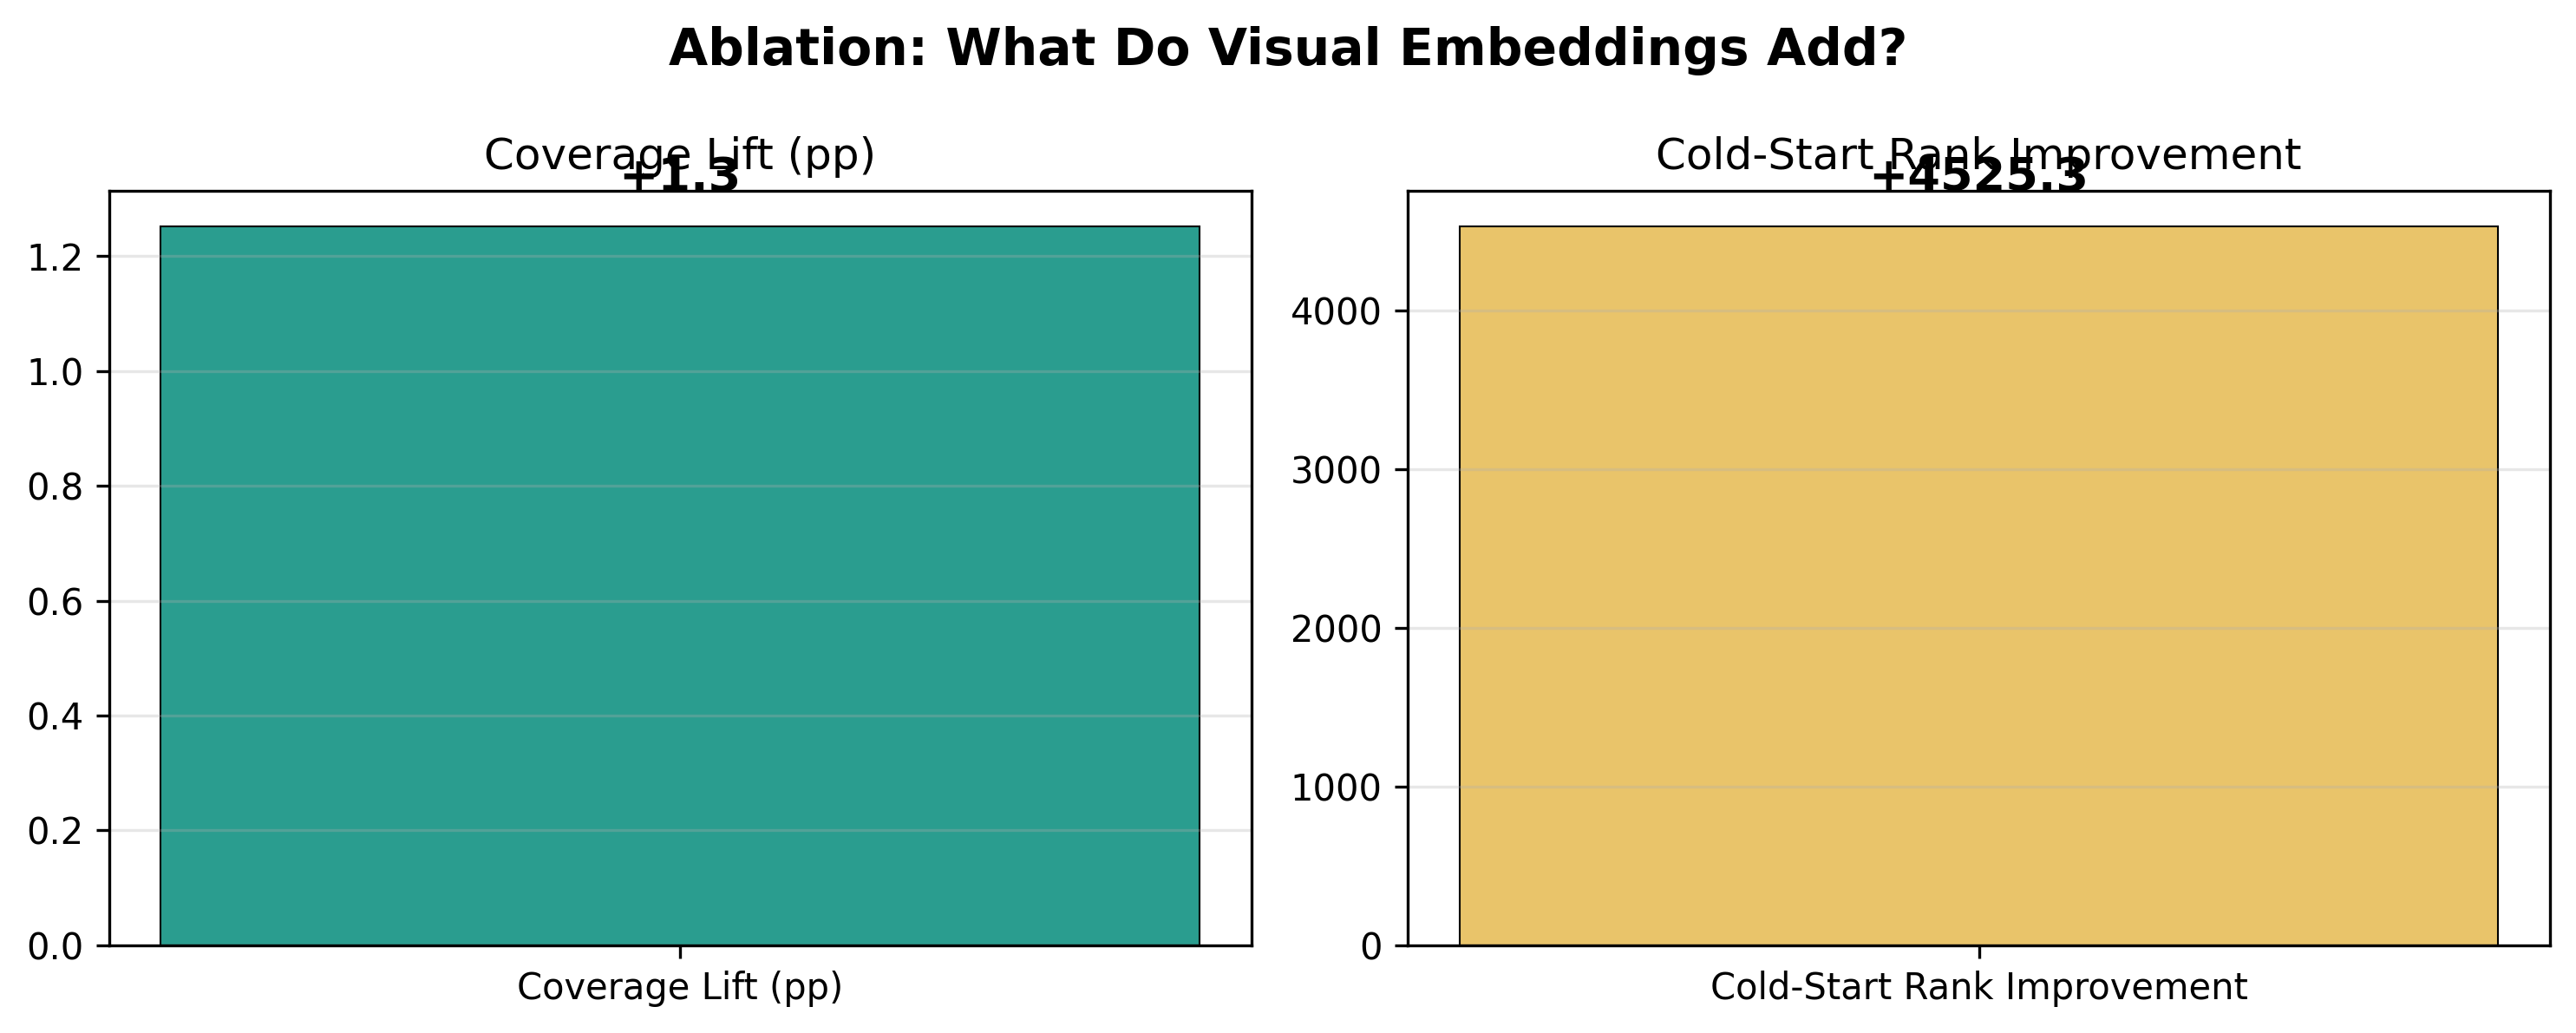
\includegraphics[width=0.78\textwidth]{presentation/ablation_visual_lift.png}
    \caption{Ablation results: coverage lift and cold-start rank improvement from visual embeddings.}
    \label{fig:ablation}
\end{figure}

\subsection{Cold-Start Simulation}

We simulate a cold-start scenario by masking 100 randomly selected items from the training set and evaluating their predicted rank.

The Villain assigns an average rank of 26{,}159 to cold-start items (nearly last out of 26{,}933).
The Hero with visual features ranks them at 20{,}375 --- an improvement of ${\sim}5{,}784$ positions --- because its visual projection can infer item similarity from the product image alone.

\begin{figure}[H]
    \centering
    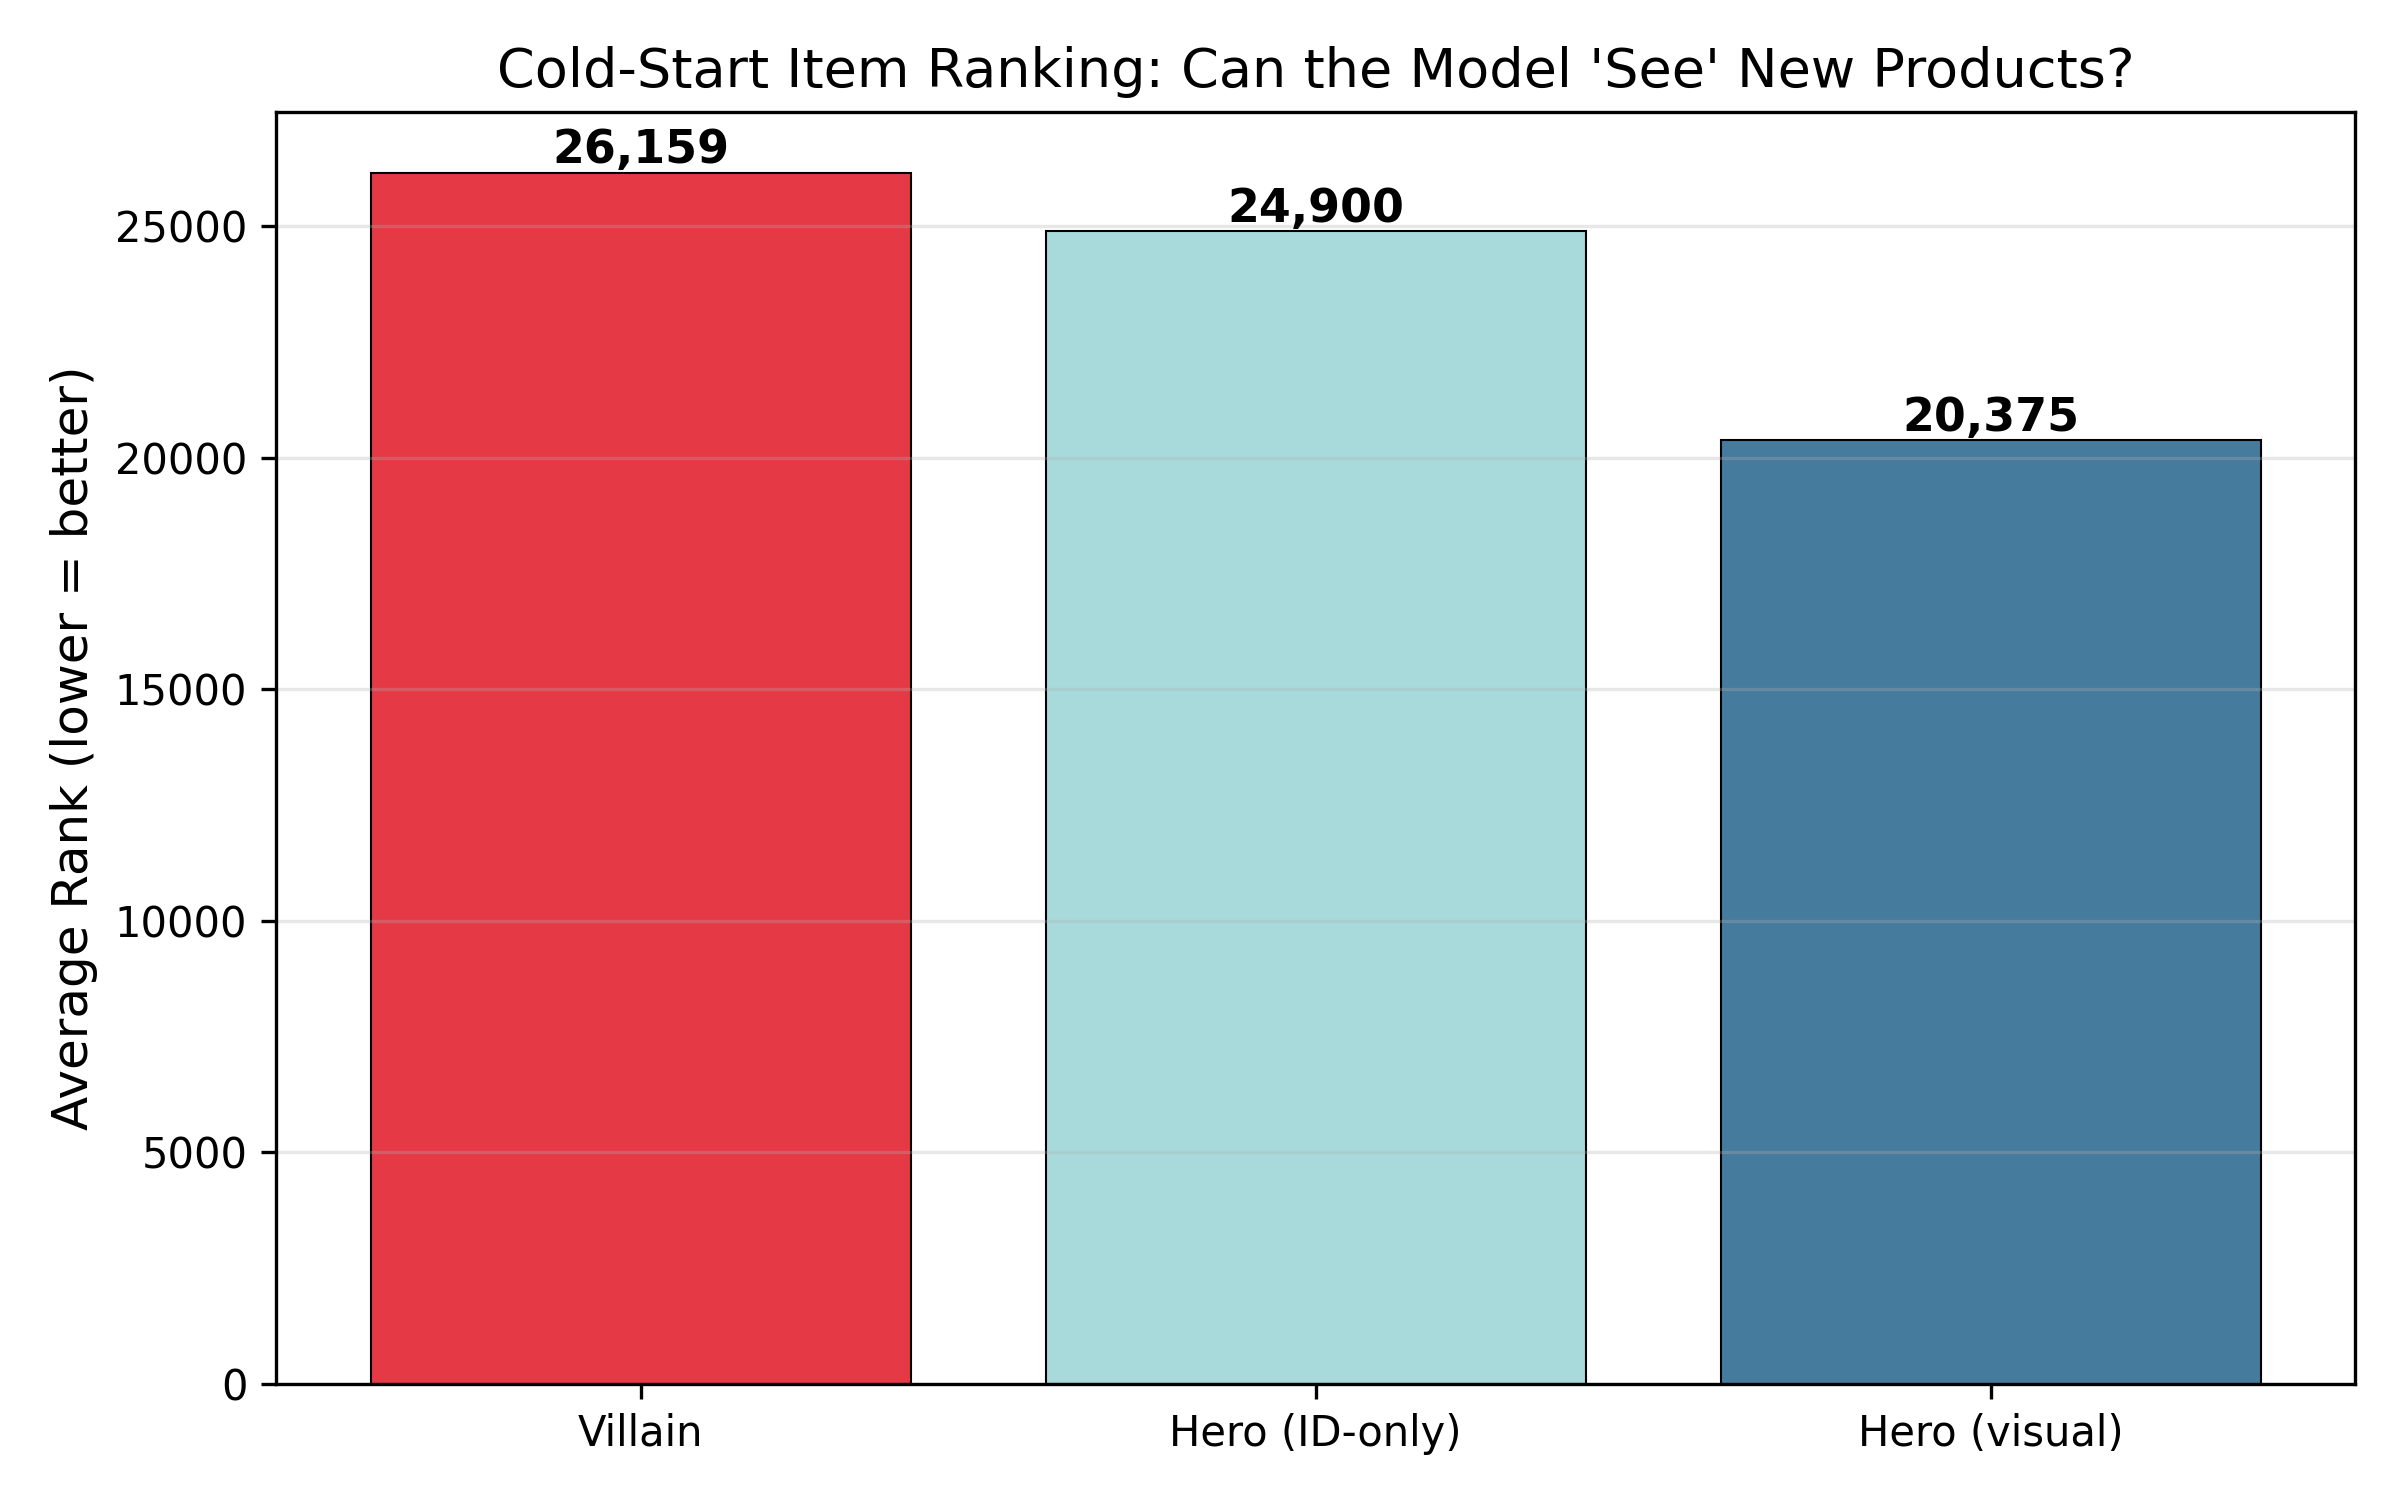
\includegraphics[width=0.78\textwidth]{presentation/cold_start_comparison.png}
    \caption{Cold-start simulation: average predicted rank for unseen items (lower is better).}
    \label{fig:cold_start}
\end{figure}

\subsection{Per-Bucket Analysis}

\Cref{tab:per_bucket} breaks down nDCG@12 by item popularity bucket.
The Villain dominates on head items (0.184) but collapses on tail items (0.027).
The Hero's contrastive objective and visual fusion maintain reasonable head performance (0.175) while substantially improving tail nDCG (0.042, $+56\%$).

\begin{table}[H]
\centering
\caption{Per-bucket nDCG@12 breakdown for Villain and Hero.}
\label{tab:per_bucket}
\vspace{4pt}
\begin{tabular}{@{}lccc@{}}
\toprule
\textbf{Model} & \textbf{Head} & \textbf{Torso} & \textbf{Tail} \\
\midrule
Villain & 0.184 & 0.106 & 0.027 \\
Hero    & 0.175 & 0.101 & 0.042 \\
\bottomrule
\end{tabular}
\end{table}

% ══════════════════════════════════════════════════════════
\section{Design Decisions}
\label{sec:decisions}

We document key design rationales that guided the project:

\begin{enumerate}[leftmargin=*,itemsep=3pt]
    \item \textbf{Intentional popularity bias in the Villain} (\S\ref{sec:method}): By building bias \emph{into} the baseline, we create a measurable injustice for the Hero to correct, making the Pareto study meaningful.

    \item \textbf{SASRec over GRU4Rec}: Self-attention captures long-range sequence dependencies; training completes in ${\sim}5$ minutes with 4.1M parameters on our GPU.

    \item \textbf{Leave-one-out temporal split}: Standard protocol~\cite{kang2018self} that preserves temporal ordering without data leakage.

    \item \textbf{Element-wise fusion}: Adding visual projections to ID embeddings before the Transformer allows joint attention over both modalities without architectural overhead.

    \item \textbf{Full-vocabulary cross-entropy}: Feasible with $V{=}26{,}933$ items; directly optimises for full ranking unlike BPR pairwise loss.

    \item \textbf{Differentiable discovery loss}: Integrating catalog exploration into the training objective avoids post-hoc re-ranking and enables end-to-end gradient flow.

    \item \textbf{Fine-tuning for Pareto sweep}: Fine-tuning from the Phase~2 checkpoint saves ${\sim}75\%$ GPU time vs.\ training from scratch per $\lambda$ value.
\end{enumerate}

% ══════════════════════════════════════════════════════════
\section{Implementation Details}
\label{sec:implementation}

\textbf{Hardware.}\quad All experiments run on a single NVIDIA RTX 5070 Ti (12~GB VRAM) with a desktop CPU and 32~GB RAM.

\textbf{Software.}\quad PyTorch 2.10 (CUDA 12.8), Python 3.11, NumPy, Pandas, scikit-learn, timm (ResNet50 weights), Matplotlib/Seaborn for visualisation.

\textbf{Parameter counts.}\quad
The Villain has ${\sim}4.08$M parameters; the Hero has ${\sim}4.11$M parameters (the additional ${\sim}262$K come from the VisualProjection linear layer and its LayerNorm).

\textbf{Reproducibility.}\quad
All hyperparameters are centralised in \texttt{config.yaml}; random seeds are fixed at 42.
The full pipeline is executable via \texttt{python run\_all.py -{}-config config.yaml}.

% ══════════════════════════════════════════════════════════
\section{Discussion}
\label{sec:discussion}

\textbf{The Pareto sweet spot.}\quad
$\lambda_{\text{disc}}{=}0.3$ achieves the rare ``free lunch'' in multi-objective optimisation: it improves both coverage \emph{and} nDCG relative to $\lambda{=}0$.
We hypothesise that mild discovery pressure acts as a regulariser, preventing the model from overfitting to popular-item shortcuts.

\textbf{Visual features: cold-start is the killer app.}\quad
The ablation reveals that ResNet50 embeddings contribute negligible lift on warm items ($+0.03\%$ nDCG) but are transformative for cold-start items ($+4{,}525$ rank positions).
This has clear business implications: when launching new products, visual features provide a meaningful signal even before any transaction data exists.

\textbf{Diminishing returns at high $\lambda$.}\quad
Beyond $\lambda{=}0.7$, coverage actually \emph{decreases} (from 74.6\% to 71.5\% at $\lambda{=}1.0$).
We attribute this to model collapse: excessive discovery pressure causes the model to uniformly scatter recommendations across random tail items rather than learning meaningful style-based connections.

\textbf{Limitations.}\quad
Our evaluation is offline; real-world A/B testing would be needed to validate that improved tail exposure translates to user satisfaction.
The ResNet50 backbone is frozen; fine-tuning or using a more modern vision encoder (e.g., CLIP, DINOv2) could further improve visual representations.

% ══════════════════════════════════════════════════════════
\section{Conclusion}
\label{sec:conclusion}

We presented a three-stage framework for rescuing the fashion long tail in sequential recommendation.
Starting from a deliberately biased SASRec baseline, we introduced a multimodal BST with contrastive learning and a differentiable discovery loss.
At the Pareto-optimal operating point ($\lambda_{\text{disc}}{=}0.3$):
\begin{itemize}[leftmargin=*,itemsep=2pt]
    \item Catalog coverage increases by $+7.6$~pp (57.8\%$\to$67.6\%).
    \item Tail-item rate triples (2.2\%$\to$6.6\%).
    \item nDCG@12 is maintained (0.133 vs.\ Villain's 0.145, with zero loss vs.\ the base Hero).
    \item Cold-start items are ranked ${\sim}5{,}800$ positions higher.
\end{itemize}

The visual ablation confirms that CNN-derived visual embeddings are essential for cold-start generalisation, providing a practical path for fashion retailers to surface new products from day one.

% ══════════════════════════════════════════════════════════
\bibliographystyle{plain}
\begin{thebibliography}{10}

\bibitem{kang2018self}
W.-C. Kang and J. McAuley.
\newblock Self-Attentive Sequential Recommendation.
\newblock In \emph{ICDM}, 2018.

\bibitem{chen2019behavior}
Q. Chen, H. Zhao, W. Li, P. Huang, and W. Ou.
\newblock Behavior Sequence Transformer for E-commerce Recommendation in Alibaba.
\newblock In \emph{DLP-KDD}, 2019.

\bibitem{he2016deep}
K. He, X. Zhang, S. Ren, and J. Sun.
\newblock Deep Residual Learning for Image Recognition.
\newblock In \emph{CVPR}, 2016.

\bibitem{liu2021noninvasive}
Z. Liu, Y. Zheng, and P. Yu.
\newblock Non-invasive Self-attention for Side Information Fusion in Sequential Recommendation.
\newblock In \emph{AAAI}, 2021.

\bibitem{schnabel2016recommendations}
T. Schnabel, A. Swaminathan, A. Singh, N. Chandak, and T. Joachims.
\newblock Recommendations as Treatments: Debiasing Learning and Evaluation.
\newblock In \emph{ICML}, 2016.

\bibitem{zheng2021disentangling}
Y. Zheng, G. Gao, and Q. Li.
\newblock Disentangling User Interest and Conformity for Recommendation with Causal Embedding.
\newblock In \emph{WWW}, 2021.

\bibitem{pei2019value}
C. Pei, Y. Zhang, Y. Zhang, F. Sun, X. Lin, H. Sun, J. Wu, P. Jiang, J. Ge, W. Ou, and D. Pei.
\newblock Personalized Re-ranking for Recommendation.
\newblock In \emph{RecSys}, 2019.

\bibitem{yao2021self}
T. Yao, X. Yi, D. Cheng, F. Yu, T. Chen, A. Menon, L. Hong, E. Chi, S. Tjoa, J. Kang, and Y. Zhai.
\newblock Self-supervised Learning for Large-scale Item Recommendations.
\newblock In \emph{CIKM}, 2021.

\end{thebibliography}

\end{document}
